% Created by tikzDevice version 0.7.0 on 2014-06-29 19:47:56
% !TEX encoding = UTF-8 Unicode
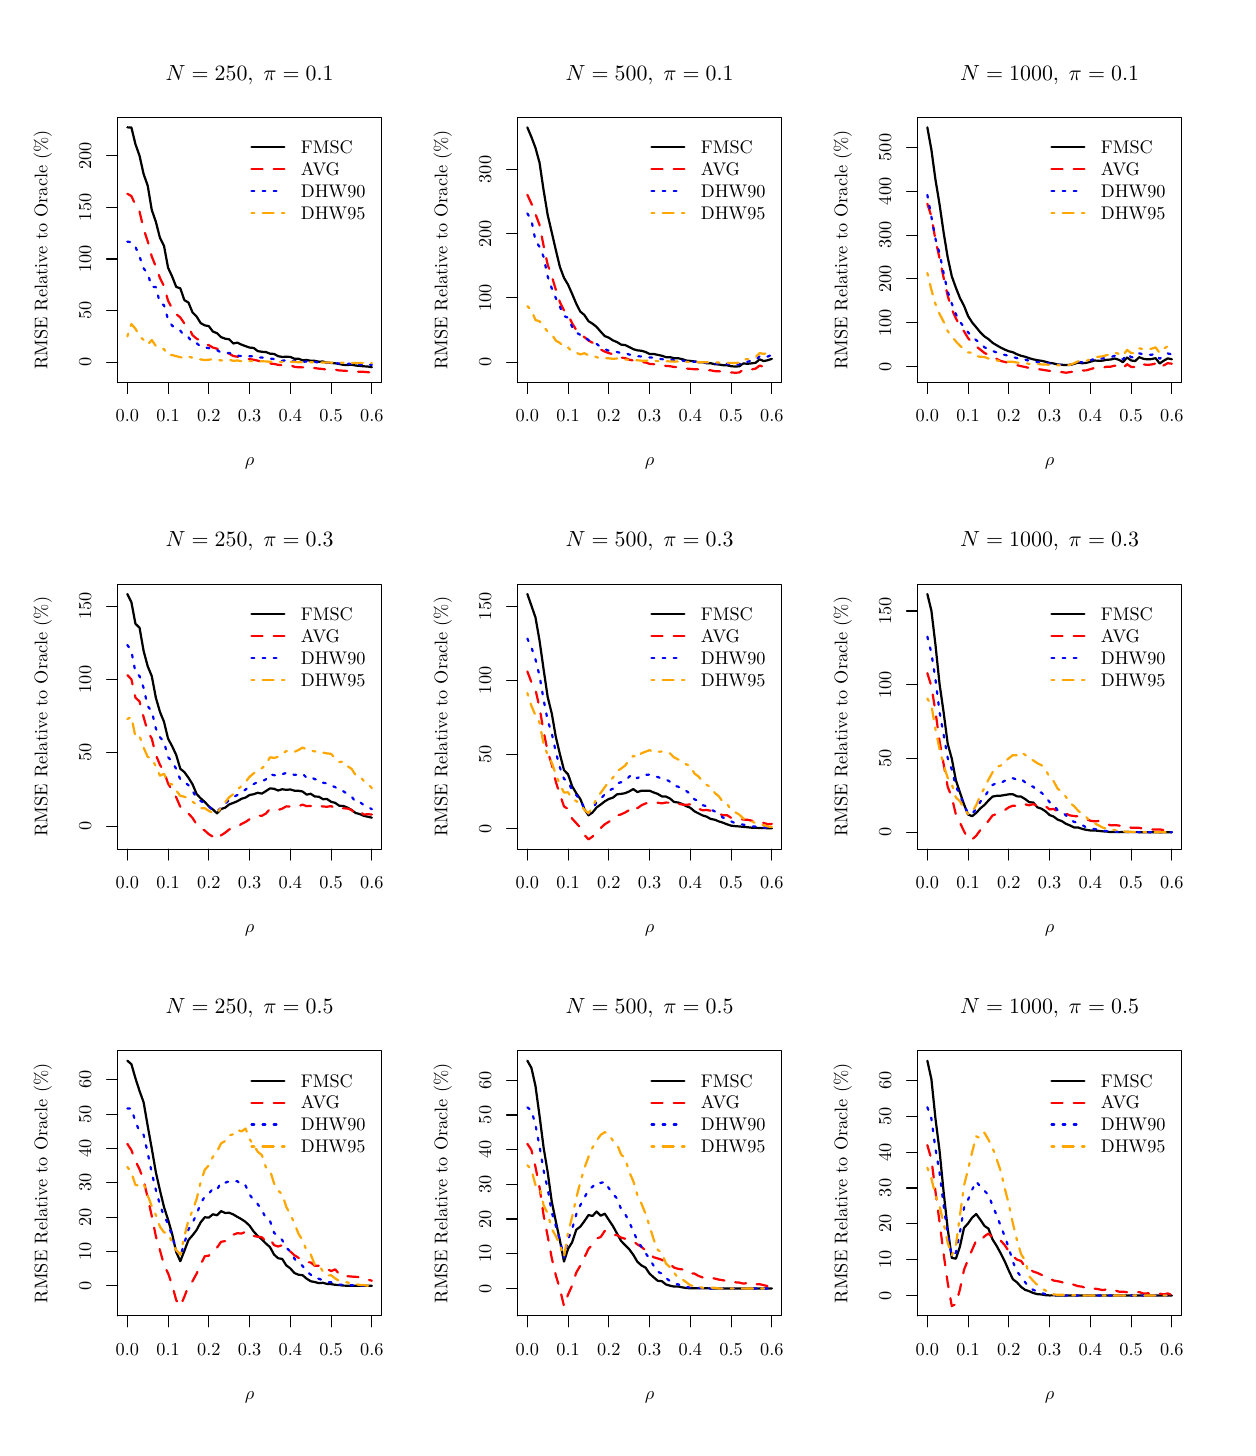
\begin{tikzpicture}[x=1pt,y=1pt]
\definecolor[named]{fillColor}{rgb}{1.00,1.00,1.00}
\path[use as bounding box,fill=fillColor,fill opacity=0.00] (0,0) rectangle (433.62,505.89);
\begin{scope}
\path[clip] ( 32.47,377.65) rectangle (127.91,473.42);
\definecolor[named]{drawColor}{rgb}{0.00,0.00,0.00}

\path[draw=drawColor,line width= 0.8pt,line join=round,line cap=round] ( 36.01,469.87) --
	( 37.48,469.80) --
	( 38.95,463.76) --
	( 40.42,459.61) --
	( 41.90,452.96) --
	( 43.37,448.82) --
	( 44.84,440.04) --
	( 46.32,435.74) --
	( 47.79,429.97) --
	( 49.26,427.06) --
	( 50.73,419.14) --
	( 52.21,415.95) --
	( 53.68,412.20) --
	( 55.15,411.72) --
	( 56.63,407.42) --
	( 58.10,406.57) --
	( 59.57,402.98) --
	( 61.04,401.51) --
	( 62.52,399.12) --
	( 63.99,398.32) --
	( 65.46,398.04) --
	( 66.93,396.08) --
	( 68.41,395.50) --
	( 69.88,394.06) --
	( 71.35,393.51) --
	( 72.83,393.26) --
	( 74.30,391.77) --
	( 75.77,392.08) --
	( 77.24,391.36) --
	( 78.72,390.80) --
	( 80.19,390.29) --
	( 81.66,390.16) --
	( 83.14,389.01) --
	( 84.61,388.76) --
	( 86.08,388.68) --
	( 87.55,388.09) --
	( 89.03,387.99) --
	( 90.50,387.18) --
	( 91.97,386.91) --
	( 93.44,386.97) --
	( 94.92,386.91) --
	( 96.39,386.25) --
	( 97.86,386.27) --
	( 99.34,385.70) --
	(100.81,385.80) --
	(102.28,385.53) --
	(103.75,385.49) --
	(105.23,385.18) --
	(106.70,385.25) --
	(108.17,384.80) --
	(109.65,384.75) --
	(111.12,384.60) --
	(112.59,384.35) --
	(114.06,384.05) --
	(115.54,383.97) --
	(117.01,384.11) --
	(118.48,383.81) --
	(119.95,383.67) --
	(121.43,383.52) --
	(122.90,383.44) --
	(124.37,383.20);
\end{scope}
\begin{scope}
\path[clip] (  0.00,  0.00) rectangle (433.62,505.89);
\definecolor[named]{drawColor}{rgb}{0.00,0.00,0.00}

\path[draw=drawColor,line width= 0.4pt,line join=round,line cap=round] ( 36.01,377.65) -- (124.37,377.65);

\path[draw=drawColor,line width= 0.4pt,line join=round,line cap=round] ( 36.01,377.65) -- ( 36.01,373.69);

\path[draw=drawColor,line width= 0.4pt,line join=round,line cap=round] ( 50.73,377.65) -- ( 50.73,373.69);

\path[draw=drawColor,line width= 0.4pt,line join=round,line cap=round] ( 65.46,377.65) -- ( 65.46,373.69);

\path[draw=drawColor,line width= 0.4pt,line join=round,line cap=round] ( 80.19,377.65) -- ( 80.19,373.69);

\path[draw=drawColor,line width= 0.4pt,line join=round,line cap=round] ( 94.92,377.65) -- ( 94.92,373.69);

\path[draw=drawColor,line width= 0.4pt,line join=round,line cap=round] (109.65,377.65) -- (109.65,373.69);

\path[draw=drawColor,line width= 0.4pt,line join=round,line cap=round] (124.37,377.65) -- (124.37,373.69);

\node[text=drawColor,anchor=base,inner sep=0pt, outer sep=0pt, scale=  0.66] at ( 36.01,363.40) {0.0};

\node[text=drawColor,anchor=base,inner sep=0pt, outer sep=0pt, scale=  0.66] at ( 50.73,363.40) {0.1};

\node[text=drawColor,anchor=base,inner sep=0pt, outer sep=0pt, scale=  0.66] at ( 65.46,363.40) {0.2};

\node[text=drawColor,anchor=base,inner sep=0pt, outer sep=0pt, scale=  0.66] at ( 80.19,363.40) {0.3};

\node[text=drawColor,anchor=base,inner sep=0pt, outer sep=0pt, scale=  0.66] at ( 94.92,363.40) {0.4};

\node[text=drawColor,anchor=base,inner sep=0pt, outer sep=0pt, scale=  0.66] at (109.65,363.40) {0.5};

\node[text=drawColor,anchor=base,inner sep=0pt, outer sep=0pt, scale=  0.66] at (124.37,363.40) {0.6};

\path[draw=drawColor,line width= 0.4pt,line join=round,line cap=round] ( 32.47,384.95) -- ( 32.47,459.63);

\path[draw=drawColor,line width= 0.4pt,line join=round,line cap=round] ( 32.47,384.95) -- ( 28.51,384.95);

\path[draw=drawColor,line width= 0.4pt,line join=round,line cap=round] ( 32.47,403.62) -- ( 28.51,403.62);

\path[draw=drawColor,line width= 0.4pt,line join=round,line cap=round] ( 32.47,422.29) -- ( 28.51,422.29);

\path[draw=drawColor,line width= 0.4pt,line join=round,line cap=round] ( 32.47,440.96) -- ( 28.51,440.96);

\path[draw=drawColor,line width= 0.4pt,line join=round,line cap=round] ( 32.47,459.63) -- ( 28.51,459.63);

\node[text=drawColor,rotate= 90.00,anchor=base,inner sep=0pt, outer sep=0pt, scale=  0.66] at ( 22.97,384.95) {0};

\node[text=drawColor,rotate= 90.00,anchor=base,inner sep=0pt, outer sep=0pt, scale=  0.66] at ( 22.97,403.62) {50};

\node[text=drawColor,rotate= 90.00,anchor=base,inner sep=0pt, outer sep=0pt, scale=  0.66] at ( 22.97,422.29) {100};

\node[text=drawColor,rotate= 90.00,anchor=base,inner sep=0pt, outer sep=0pt, scale=  0.66] at ( 22.97,440.96) {150};

\node[text=drawColor,rotate= 90.00,anchor=base,inner sep=0pt, outer sep=0pt, scale=  0.66] at ( 22.97,459.63) {200};

\path[draw=drawColor,line width= 0.4pt,line join=round,line cap=round] ( 32.47,377.65) --
	(127.91,377.65) --
	(127.91,473.42) --
	( 32.47,473.42) --
	( 32.47,377.65);
\end{scope}
\begin{scope}
\path[clip] (  0.00,337.26) rectangle (144.54,505.89);
\definecolor[named]{drawColor}{rgb}{0.00,0.00,0.00}

\node[text=drawColor,anchor=base,inner sep=0pt, outer sep=0pt, scale=  0.79] at ( 80.19,486.92) {\bfseries $N=250, \;\pi=0.1$};

\node[text=drawColor,anchor=base,inner sep=0pt, outer sep=0pt, scale=  0.66] at ( 80.19,347.56) {$\rho$};

\node[text=drawColor,rotate= 90.00,anchor=base,inner sep=0pt, outer sep=0pt, scale=  0.66] at (  7.13,425.53) {RMSE Relative to Oracle (\%)};
\end{scope}
\begin{scope}
\path[clip] ( 32.47,377.65) rectangle (127.91,473.42);
\definecolor[named]{drawColor}{rgb}{1.00,0.00,0.00}

\path[draw=drawColor,line width= 0.8pt,dash pattern=on 4pt off 4pt ,line join=round,line cap=round] ( 36.01,445.88) --
	( 37.48,445.03) --
	( 38.95,441.80) --
	( 40.42,439.45) --
	( 41.90,433.10) --
	( 43.37,428.76) --
	( 44.84,423.19) --
	( 46.32,419.49) --
	( 47.79,415.46) --
	( 49.26,412.45) --
	( 50.73,407.20) --
	( 52.21,404.41) --
	( 53.68,402.36) --
	( 55.15,401.17) --
	( 56.63,398.99) --
	( 58.10,397.80) --
	( 59.57,394.77) --
	( 61.04,393.50) --
	( 62.52,392.79) --
	( 63.99,391.71) --
	( 65.46,391.15) --
	( 66.93,390.28) --
	( 68.41,389.88) --
	( 69.88,388.88) --
	( 71.35,388.53) --
	( 72.83,388.08) --
	( 74.30,387.24) --
	( 75.77,386.99) --
	( 77.24,387.01) --
	( 78.72,386.19) --
	( 80.19,386.12) --
	( 81.66,385.90) --
	( 83.14,385.56) --
	( 84.61,385.06) --
	( 86.08,384.74) --
	( 87.55,384.53) --
	( 89.03,384.38) --
	( 90.50,384.06) --
	( 91.97,383.91) --
	( 93.44,383.74) --
	( 94.92,383.85) --
	( 96.39,383.34) --
	( 97.86,383.17) --
	( 99.34,383.13) --
	(100.81,383.29) --
	(102.28,382.99) --
	(103.75,382.88) --
	(105.23,382.67) --
	(106.70,382.54) --
	(108.17,382.27) --
	(109.65,382.28) --
	(111.12,382.30) --
	(112.59,382.01) --
	(114.06,381.94) --
	(115.54,381.84) --
	(117.01,381.81) --
	(118.48,381.59) --
	(119.95,381.54) --
	(121.43,381.52) --
	(122.90,381.40) --
	(124.37,381.20);
\definecolor[named]{drawColor}{rgb}{0.00,0.00,1.00}

\path[draw=drawColor,line width= 0.8pt,dash pattern=on 1pt off 3pt ,line join=round,line cap=round] ( 36.01,428.57) --
	( 37.48,428.37) --
	( 38.95,426.66) --
	( 40.42,423.17) --
	( 41.90,418.92) --
	( 43.37,416.97) --
	( 44.84,412.27) --
	( 46.32,412.13) --
	( 47.79,406.33) --
	( 49.26,405.62) --
	( 50.73,400.42) --
	( 52.21,398.19) --
	( 53.68,397.12) --
	( 55.15,396.40) --
	( 56.63,394.50) --
	( 58.10,394.01) --
	( 59.57,392.03) --
	( 61.04,391.86) --
	( 62.52,390.70) --
	( 63.99,390.40) --
	( 65.46,390.08) --
	( 66.93,389.95) --
	( 68.41,389.36) --
	( 69.88,388.51) --
	( 71.35,388.39) --
	( 72.83,388.34) --
	( 74.30,387.60) --
	( 75.77,387.35) --
	( 77.24,387.24) --
	( 78.72,387.35) --
	( 80.19,387.17) --
	( 81.66,387.15) --
	( 83.14,386.61) --
	( 84.61,386.69) --
	( 86.08,386.48) --
	( 87.55,386.28) --
	( 89.03,386.17) --
	( 90.50,385.90) --
	( 91.97,385.53) --
	( 93.44,385.72) --
	( 94.92,385.67) --
	( 96.39,385.43) --
	( 97.86,385.41) --
	( 99.34,385.12) --
	(100.81,385.26) --
	(102.28,384.99) --
	(103.75,385.09) --
	(105.23,384.87) --
	(106.70,384.87) --
	(108.17,384.77) --
	(109.65,384.77) --
	(111.12,384.66) --
	(112.59,384.53) --
	(114.06,384.46) --
	(115.54,384.44) --
	(117.01,384.38) --
	(118.48,384.23) --
	(119.95,384.19) --
	(121.43,384.20) --
	(122.90,384.16) --
	(124.37,384.04);
\definecolor[named]{drawColor}{rgb}{1.00,0.65,0.00}

\path[draw=drawColor,line width= 0.8pt,dash pattern=on 1pt off 3pt on 4pt off 3pt ,line join=round,line cap=round] ( 36.01,394.33) --
	( 37.48,398.79) --
	( 38.95,397.08) --
	( 40.42,394.38) --
	( 41.90,393.04) --
	( 43.37,391.35) --
	( 44.84,393.03) --
	( 46.32,390.85) --
	( 47.79,390.00) --
	( 49.26,389.72) --
	( 50.73,387.47) --
	( 52.21,387.60) --
	( 53.68,387.17) --
	( 55.15,386.83) --
	( 56.63,386.43) --
	( 58.10,386.99) --
	( 59.57,386.64) --
	( 61.04,386.12) --
	( 62.52,386.01) --
	( 63.99,385.78) --
	( 65.46,385.90) --
	( 66.93,386.10) --
	( 68.41,385.95) --
	( 69.88,385.63) --
	( 71.35,385.86) --
	( 72.83,385.87) --
	( 74.30,385.49) --
	( 75.77,385.62) --
	( 77.24,385.38) --
	( 78.72,385.38) --
	( 80.19,385.42) --
	( 81.66,385.42) --
	( 83.14,385.20) --
	( 84.61,385.33) --
	( 86.08,385.29) --
	( 87.55,385.17) --
	( 89.03,385.09) --
	( 90.50,385.17) --
	( 91.97,385.07) --
	( 93.44,385.06) --
	( 94.92,385.14) --
	( 96.39,385.14) --
	( 97.86,384.98) --
	( 99.34,384.98) --
	(100.81,384.97) --
	(102.28,384.97) --
	(103.75,384.96) --
	(105.23,384.87) --
	(106.70,384.87) --
	(108.17,384.90) --
	(109.65,384.84) --
	(111.12,384.83) --
	(112.59,384.81) --
	(114.06,384.83) --
	(115.54,384.79) --
	(117.01,384.74) --
	(118.48,384.76) --
	(119.95,384.76) --
	(121.43,384.76) --
	(122.90,384.67) --
	(124.37,384.67);
\definecolor[named]{drawColor}{rgb}{0.00,0.00,0.00}

\path[draw=drawColor,line width= 0.8pt,line join=round,line cap=round] ( 80.89,462.63) -- ( 92.77,462.63);
\definecolor[named]{drawColor}{rgb}{1.00,0.00,0.00}

\path[draw=drawColor,line width= 0.8pt,dash pattern=on 4pt off 4pt ,line join=round,line cap=round] ( 80.89,454.71) -- ( 92.77,454.71);
\definecolor[named]{drawColor}{rgb}{0.00,0.00,1.00}

\path[draw=drawColor,line width= 0.8pt,dash pattern=on 1pt off 3pt ,line join=round,line cap=round] ( 80.89,446.79) -- ( 92.77,446.79);
\definecolor[named]{drawColor}{rgb}{1.00,0.65,0.00}

\path[draw=drawColor,line width= 0.8pt,dash pattern=on 1pt off 3pt on 4pt off 3pt ,line join=round,line cap=round] ( 80.89,438.87) -- ( 92.77,438.87);
\definecolor[named]{drawColor}{rgb}{0.00,0.00,0.00}

\node[text=drawColor,anchor=base west,inner sep=0pt, outer sep=0pt, scale=  0.66] at ( 98.71,460.35) {FMSC};

\node[text=drawColor,anchor=base west,inner sep=0pt, outer sep=0pt, scale=  0.66] at ( 98.71,452.43) {AVG};

\node[text=drawColor,anchor=base west,inner sep=0pt, outer sep=0pt, scale=  0.66] at ( 98.71,444.51) {DHW90};

\node[text=drawColor,anchor=base west,inner sep=0pt, outer sep=0pt, scale=  0.66] at ( 98.71,436.59) {DHW95};
\end{scope}
\begin{scope}
\path[clip] (177.01,377.65) rectangle (272.45,473.42);
\definecolor[named]{drawColor}{rgb}{0.00,0.00,0.00}

\path[draw=drawColor,line width= 0.8pt,line join=round,line cap=round] (180.55,469.87) --
	(182.02,466.38) --
	(183.49,462.46) --
	(184.96,457.10) --
	(186.44,447.04) --
	(187.91,438.19) --
	(189.38,431.87) --
	(190.86,425.46) --
	(192.33,419.39) --
	(193.80,415.49) --
	(195.27,413.01) --
	(196.75,409.66) --
	(198.22,406.16) --
	(199.69,403.29) --
	(201.17,402.06) --
	(202.64,399.83) --
	(204.11,398.92) --
	(205.58,397.74) --
	(207.06,396.03) --
	(208.53,394.44) --
	(210.00,393.85) --
	(211.47,392.88) --
	(212.95,392.28) --
	(214.42,391.36) --
	(215.89,391.19) --
	(217.37,390.49) --
	(218.84,389.71) --
	(220.31,389.28) --
	(221.78,389.14) --
	(223.26,388.70) --
	(224.73,387.99) --
	(226.20,387.97) --
	(227.68,387.66) --
	(229.15,387.34) --
	(230.62,386.83) --
	(232.09,386.81) --
	(233.57,386.47) --
	(235.04,386.44) --
	(236.51,386.11) --
	(237.98,385.61) --
	(239.46,385.46) --
	(240.93,385.28) --
	(242.40,385.02) --
	(243.88,385.01) --
	(245.35,384.62) --
	(246.82,384.62) --
	(248.29,384.26) --
	(249.77,384.18) --
	(251.24,383.92) --
	(252.71,383.88) --
	(254.19,383.55) --
	(255.66,383.44) --
	(257.13,383.52) --
	(258.60,384.56) --
	(260.08,384.42) --
	(261.55,384.59) --
	(263.02,384.78) --
	(264.50,386.03) --
	(265.97,385.41) --
	(267.44,385.72) --
	(268.91,386.21);
\end{scope}
\begin{scope}
\path[clip] (  0.00,  0.00) rectangle (433.62,505.89);
\definecolor[named]{drawColor}{rgb}{0.00,0.00,0.00}

\path[draw=drawColor,line width= 0.4pt,line join=round,line cap=round] (180.55,377.65) -- (268.91,377.65);

\path[draw=drawColor,line width= 0.4pt,line join=round,line cap=round] (180.55,377.65) -- (180.55,373.69);

\path[draw=drawColor,line width= 0.4pt,line join=round,line cap=round] (195.27,377.65) -- (195.27,373.69);

\path[draw=drawColor,line width= 0.4pt,line join=round,line cap=round] (210.00,377.65) -- (210.00,373.69);

\path[draw=drawColor,line width= 0.4pt,line join=round,line cap=round] (224.73,377.65) -- (224.73,373.69);

\path[draw=drawColor,line width= 0.4pt,line join=round,line cap=round] (239.46,377.65) -- (239.46,373.69);

\path[draw=drawColor,line width= 0.4pt,line join=round,line cap=round] (254.19,377.65) -- (254.19,373.69);

\path[draw=drawColor,line width= 0.4pt,line join=round,line cap=round] (268.91,377.65) -- (268.91,373.69);

\node[text=drawColor,anchor=base,inner sep=0pt, outer sep=0pt, scale=  0.66] at (180.55,363.40) {0.0};

\node[text=drawColor,anchor=base,inner sep=0pt, outer sep=0pt, scale=  0.66] at (195.27,363.40) {0.1};

\node[text=drawColor,anchor=base,inner sep=0pt, outer sep=0pt, scale=  0.66] at (210.00,363.40) {0.2};

\node[text=drawColor,anchor=base,inner sep=0pt, outer sep=0pt, scale=  0.66] at (224.73,363.40) {0.3};

\node[text=drawColor,anchor=base,inner sep=0pt, outer sep=0pt, scale=  0.66] at (239.46,363.40) {0.4};

\node[text=drawColor,anchor=base,inner sep=0pt, outer sep=0pt, scale=  0.66] at (254.19,363.40) {0.5};

\node[text=drawColor,anchor=base,inner sep=0pt, outer sep=0pt, scale=  0.66] at (268.91,363.40) {0.6};

\path[draw=drawColor,line width= 0.4pt,line join=round,line cap=round] (177.01,385.05) -- (177.01,454.64);

\path[draw=drawColor,line width= 0.4pt,line join=round,line cap=round] (177.01,385.05) -- (173.05,385.05);

\path[draw=drawColor,line width= 0.4pt,line join=round,line cap=round] (177.01,408.25) -- (173.05,408.25);

\path[draw=drawColor,line width= 0.4pt,line join=round,line cap=round] (177.01,431.45) -- (173.05,431.45);

\path[draw=drawColor,line width= 0.4pt,line join=round,line cap=round] (177.01,454.64) -- (173.05,454.64);

\node[text=drawColor,rotate= 90.00,anchor=base,inner sep=0pt, outer sep=0pt, scale=  0.66] at (167.51,385.05) {0};

\node[text=drawColor,rotate= 90.00,anchor=base,inner sep=0pt, outer sep=0pt, scale=  0.66] at (167.51,408.25) {100};

\node[text=drawColor,rotate= 90.00,anchor=base,inner sep=0pt, outer sep=0pt, scale=  0.66] at (167.51,431.45) {200};

\node[text=drawColor,rotate= 90.00,anchor=base,inner sep=0pt, outer sep=0pt, scale=  0.66] at (167.51,454.64) {300};

\path[draw=drawColor,line width= 0.4pt,line join=round,line cap=round] (177.01,377.65) --
	(272.45,377.65) --
	(272.45,473.42) --
	(177.01,473.42) --
	(177.01,377.65);
\end{scope}
\begin{scope}
\path[clip] (144.54,337.26) rectangle (289.08,505.89);
\definecolor[named]{drawColor}{rgb}{0.00,0.00,0.00}

\node[text=drawColor,anchor=base,inner sep=0pt, outer sep=0pt, scale=  0.79] at (224.73,486.92) {\bfseries $N=500, \;\pi=0.1$};

\node[text=drawColor,anchor=base,inner sep=0pt, outer sep=0pt, scale=  0.66] at (224.73,347.56) {$\rho$};

\node[text=drawColor,rotate= 90.00,anchor=base,inner sep=0pt, outer sep=0pt, scale=  0.66] at (151.67,425.53) {RMSE Relative to Oracle (\%)};
\end{scope}
\begin{scope}
\path[clip] (177.01,377.65) rectangle (272.45,473.42);
\definecolor[named]{drawColor}{rgb}{1.00,0.00,0.00}

\path[draw=drawColor,line width= 0.8pt,dash pattern=on 4pt off 4pt ,line join=round,line cap=round] (180.55,445.51) --
	(182.02,442.34) --
	(183.49,438.55) --
	(184.96,434.60) --
	(186.44,426.98) --
	(187.91,420.20) --
	(189.38,416.10) --
	(190.86,411.13) --
	(192.33,406.68) --
	(193.80,403.72) --
	(195.27,402.12) --
	(196.75,399.05) --
	(198.22,396.69) --
	(199.69,395.07) --
	(201.17,394.07) --
	(202.64,392.84) --
	(204.11,392.02) --
	(205.58,390.82) --
	(207.06,389.56) --
	(208.53,388.83) --
	(210.00,388.29) --
	(211.47,387.86) --
	(212.95,387.21) --
	(214.42,386.66) --
	(215.89,386.49) --
	(217.37,385.91) --
	(218.84,385.59) --
	(220.31,385.19) --
	(221.78,384.94) --
	(223.26,384.93) --
	(224.73,384.38) --
	(226.20,384.29) --
	(227.68,384.09) --
	(229.15,383.85) --
	(230.62,383.66) --
	(232.09,383.56) --
	(233.57,383.28) --
	(235.04,383.21) --
	(236.51,382.97) --
	(237.98,382.72) --
	(239.46,382.59) --
	(240.93,382.46) --
	(242.40,382.43) --
	(243.88,382.35) --
	(245.35,382.05) --
	(246.82,382.06) --
	(248.29,381.76) --
	(249.77,381.71) --
	(251.24,381.60) --
	(252.71,381.49) --
	(254.19,381.29) --
	(255.66,381.20) --
	(257.13,381.27) --
	(258.60,382.37) --
	(260.08,382.18) --
	(261.55,382.37) --
	(263.02,382.68) --
	(264.50,383.79) --
	(265.97,383.33) --
	(267.44,383.63) --
	(268.91,384.08);
\definecolor[named]{drawColor}{rgb}{0.00,0.00,1.00}

\path[draw=drawColor,line width= 0.8pt,dash pattern=on 1pt off 3pt ,line join=round,line cap=round] (180.55,438.76) --
	(182.02,436.37) --
	(183.49,428.88) --
	(184.96,426.69) --
	(186.44,423.04) --
	(187.91,415.95) --
	(189.38,411.67) --
	(190.86,408.11) --
	(192.33,404.95) --
	(193.80,401.68) --
	(195.27,401.05) --
	(196.75,397.78) --
	(198.22,395.72) --
	(199.69,394.89) --
	(201.17,394.47) --
	(202.64,392.98) --
	(204.11,392.15) --
	(205.58,391.63) --
	(207.06,390.44) --
	(208.53,389.72) --
	(210.00,389.14) --
	(211.47,388.92) --
	(212.95,388.68) --
	(214.42,388.30) --
	(215.89,388.29) --
	(217.37,387.77) --
	(218.84,387.47) --
	(220.31,387.16) --
	(221.78,387.08) --
	(223.26,386.94) --
	(224.73,386.73) --
	(226.20,386.62) --
	(227.68,386.26) --
	(229.15,386.11) --
	(230.62,386.02) --
	(232.09,385.88) --
	(233.57,385.75) --
	(235.04,385.65) --
	(236.51,385.61) --
	(237.98,385.30) --
	(239.46,385.23) --
	(240.93,385.17) --
	(242.40,385.05) --
	(243.88,385.03) --
	(245.35,384.75) --
	(246.82,384.74) --
	(248.29,384.49) --
	(249.77,384.47) --
	(251.24,384.35) --
	(252.71,384.32) --
	(254.19,384.18) --
	(255.66,384.10) --
	(257.13,384.24) --
	(258.60,385.40) --
	(260.08,385.14) --
	(261.55,385.59) --
	(263.02,385.82) --
	(264.50,387.16) --
	(265.97,386.68) --
	(267.44,387.06) --
	(268.91,387.64);
\definecolor[named]{drawColor}{rgb}{1.00,0.65,0.00}

\path[draw=drawColor,line width= 0.8pt,dash pattern=on 1pt off 3pt on 4pt off 3pt ,line join=round,line cap=round] (180.55,405.29) --
	(182.02,403.83) --
	(183.49,400.23) --
	(184.96,399.81) --
	(186.44,397.79) --
	(187.91,396.09) --
	(189.38,395.06) --
	(190.86,392.80) --
	(192.33,391.94) --
	(193.80,390.47) --
	(195.27,390.29) --
	(196.75,388.83) --
	(198.22,388.41) --
	(199.69,387.80) --
	(201.17,388.25) --
	(202.64,387.48) --
	(204.11,387.40) --
	(205.58,386.82) --
	(207.06,386.36) --
	(208.53,386.52) --
	(210.00,386.39) --
	(211.47,386.25) --
	(212.95,386.32) --
	(214.42,385.82) --
	(215.89,385.94) --
	(217.37,385.92) --
	(218.84,385.75) --
	(220.31,385.70) --
	(221.78,385.56) --
	(223.26,385.53) --
	(224.73,385.66) --
	(226.20,385.57) --
	(227.68,385.40) --
	(229.15,385.37) --
	(230.62,385.36) --
	(232.09,385.29) --
	(233.57,385.20) --
	(235.04,385.28) --
	(236.51,385.20) --
	(237.98,385.13) --
	(239.46,385.09) --
	(240.93,385.07) --
	(242.40,385.01) --
	(243.88,385.02) --
	(245.35,384.96) --
	(246.82,384.94) --
	(248.29,384.92) --
	(249.77,384.86) --
	(251.24,384.81) --
	(252.71,384.75) --
	(254.19,384.74) --
	(255.66,384.70) --
	(257.13,384.87) --
	(258.60,386.15) --
	(260.08,386.02) --
	(261.55,386.55) --
	(263.02,386.80) --
	(264.50,388.33) --
	(265.97,387.98) --
	(267.44,388.41) --
	(268.91,389.05);
\definecolor[named]{drawColor}{rgb}{0.00,0.00,0.00}

\path[draw=drawColor,line width= 0.8pt,line join=round,line cap=round] (225.43,462.63) -- (237.31,462.63);
\definecolor[named]{drawColor}{rgb}{1.00,0.00,0.00}

\path[draw=drawColor,line width= 0.8pt,dash pattern=on 4pt off 4pt ,line join=round,line cap=round] (225.43,454.71) -- (237.31,454.71);
\definecolor[named]{drawColor}{rgb}{0.00,0.00,1.00}

\path[draw=drawColor,line width= 0.8pt,dash pattern=on 1pt off 3pt ,line join=round,line cap=round] (225.43,446.79) -- (237.31,446.79);
\definecolor[named]{drawColor}{rgb}{1.00,0.65,0.00}

\path[draw=drawColor,line width= 0.8pt,dash pattern=on 1pt off 3pt on 4pt off 3pt ,line join=round,line cap=round] (225.43,438.87) -- (237.31,438.87);
\definecolor[named]{drawColor}{rgb}{0.00,0.00,0.00}

\node[text=drawColor,anchor=base west,inner sep=0pt, outer sep=0pt, scale=  0.66] at (243.25,460.35) {FMSC};

\node[text=drawColor,anchor=base west,inner sep=0pt, outer sep=0pt, scale=  0.66] at (243.25,452.43) {AVG};

\node[text=drawColor,anchor=base west,inner sep=0pt, outer sep=0pt, scale=  0.66] at (243.25,444.51) {DHW90};

\node[text=drawColor,anchor=base west,inner sep=0pt, outer sep=0pt, scale=  0.66] at (243.25,436.59) {DHW95};
\end{scope}
\begin{scope}
\path[clip] (321.55,377.65) rectangle (416.99,473.42);
\definecolor[named]{drawColor}{rgb}{0.00,0.00,0.00}

\path[draw=drawColor,line width= 0.8pt,line join=round,line cap=round] (325.09,469.87) --
	(326.56,461.75) --
	(328.03,450.92) --
	(329.50,442.07) --
	(330.98,431.83) --
	(332.45,422.87) --
	(333.92,416.06) --
	(335.40,411.93) --
	(336.87,408.21) --
	(338.34,405.40) --
	(339.81,401.68) --
	(341.29,399.37) --
	(342.76,397.59) --
	(344.23,395.79) --
	(345.71,394.34) --
	(347.18,393.36) --
	(348.65,392.02) --
	(350.12,391.14) --
	(351.60,390.28) --
	(353.07,389.57) --
	(354.54,388.96) --
	(356.01,388.61) --
	(357.49,387.87) --
	(358.96,387.32) --
	(360.43,386.98) --
	(361.91,386.44) --
	(363.38,386.03) --
	(364.85,385.72) --
	(366.32,385.51) --
	(367.80,385.17) --
	(369.27,384.76) --
	(370.74,384.55) --
	(372.22,384.15) --
	(373.69,384.07) --
	(375.16,383.96) --
	(376.63,384.01) --
	(378.11,384.37) --
	(379.58,384.86) --
	(381.05,384.62) --
	(382.52,384.77) --
	(384.00,385.17) --
	(385.47,385.60) --
	(386.94,385.54) --
	(388.42,385.57) --
	(389.89,385.86) --
	(391.36,385.97) --
	(392.83,386.33) --
	(394.31,385.87) --
	(395.78,385.00) --
	(397.25,386.72) --
	(398.73,385.62) --
	(400.20,385.43) --
	(401.67,386.82) --
	(403.14,386.24) --
	(404.62,386.03) --
	(406.09,386.12) --
	(407.56,386.47) --
	(409.04,384.54) --
	(410.51,385.55) --
	(411.98,386.38) --
	(413.45,386.07);
\end{scope}
\begin{scope}
\path[clip] (  0.00,  0.00) rectangle (433.62,505.89);
\definecolor[named]{drawColor}{rgb}{0.00,0.00,0.00}

\path[draw=drawColor,line width= 0.4pt,line join=round,line cap=round] (325.09,377.65) -- (413.45,377.65);

\path[draw=drawColor,line width= 0.4pt,line join=round,line cap=round] (325.09,377.65) -- (325.09,373.69);

\path[draw=drawColor,line width= 0.4pt,line join=round,line cap=round] (339.81,377.65) -- (339.81,373.69);

\path[draw=drawColor,line width= 0.4pt,line join=round,line cap=round] (354.54,377.65) -- (354.54,373.69);

\path[draw=drawColor,line width= 0.4pt,line join=round,line cap=round] (369.27,377.65) -- (369.27,373.69);

\path[draw=drawColor,line width= 0.4pt,line join=round,line cap=round] (384.00,377.65) -- (384.00,373.69);

\path[draw=drawColor,line width= 0.4pt,line join=round,line cap=round] (398.73,377.65) -- (398.73,373.69);

\path[draw=drawColor,line width= 0.4pt,line join=round,line cap=round] (413.45,377.65) -- (413.45,373.69);

\node[text=drawColor,anchor=base,inner sep=0pt, outer sep=0pt, scale=  0.66] at (325.09,363.40) {0.0};

\node[text=drawColor,anchor=base,inner sep=0pt, outer sep=0pt, scale=  0.66] at (339.81,363.40) {0.1};

\node[text=drawColor,anchor=base,inner sep=0pt, outer sep=0pt, scale=  0.66] at (354.54,363.40) {0.2};

\node[text=drawColor,anchor=base,inner sep=0pt, outer sep=0pt, scale=  0.66] at (369.27,363.40) {0.3};

\node[text=drawColor,anchor=base,inner sep=0pt, outer sep=0pt, scale=  0.66] at (384.00,363.40) {0.4};

\node[text=drawColor,anchor=base,inner sep=0pt, outer sep=0pt, scale=  0.66] at (398.73,363.40) {0.5};

\node[text=drawColor,anchor=base,inner sep=0pt, outer sep=0pt, scale=  0.66] at (413.45,363.40) {0.6};

\path[draw=drawColor,line width= 0.4pt,line join=round,line cap=round] (321.55,383.47) -- (321.55,462.58);

\path[draw=drawColor,line width= 0.4pt,line join=round,line cap=round] (321.55,383.47) -- (317.59,383.47);

\path[draw=drawColor,line width= 0.4pt,line join=round,line cap=round] (321.55,399.30) -- (317.59,399.30);

\path[draw=drawColor,line width= 0.4pt,line join=round,line cap=round] (321.55,415.12) -- (317.59,415.12);

\path[draw=drawColor,line width= 0.4pt,line join=round,line cap=round] (321.55,430.94) -- (317.59,430.94);

\path[draw=drawColor,line width= 0.4pt,line join=round,line cap=round] (321.55,446.76) -- (317.59,446.76);

\path[draw=drawColor,line width= 0.4pt,line join=round,line cap=round] (321.55,462.58) -- (317.59,462.58);

\node[text=drawColor,rotate= 90.00,anchor=base,inner sep=0pt, outer sep=0pt, scale=  0.66] at (312.05,383.47) {0};

\node[text=drawColor,rotate= 90.00,anchor=base,inner sep=0pt, outer sep=0pt, scale=  0.66] at (312.05,399.30) {100};

\node[text=drawColor,rotate= 90.00,anchor=base,inner sep=0pt, outer sep=0pt, scale=  0.66] at (312.05,415.12) {200};

\node[text=drawColor,rotate= 90.00,anchor=base,inner sep=0pt, outer sep=0pt, scale=  0.66] at (312.05,430.94) {300};

\node[text=drawColor,rotate= 90.00,anchor=base,inner sep=0pt, outer sep=0pt, scale=  0.66] at (312.05,446.76) {400};

\node[text=drawColor,rotate= 90.00,anchor=base,inner sep=0pt, outer sep=0pt, scale=  0.66] at (312.05,462.58) {500};

\path[draw=drawColor,line width= 0.4pt,line join=round,line cap=round] (321.55,377.65) --
	(416.99,377.65) --
	(416.99,473.42) --
	(321.55,473.42) --
	(321.55,377.65);
\end{scope}
\begin{scope}
\path[clip] (289.08,337.26) rectangle (433.62,505.89);
\definecolor[named]{drawColor}{rgb}{0.00,0.00,0.00}

\node[text=drawColor,anchor=base,inner sep=0pt, outer sep=0pt, scale=  0.79] at (369.27,486.92) {\bfseries $N=1000, \;\pi=0.1$};

\node[text=drawColor,anchor=base,inner sep=0pt, outer sep=0pt, scale=  0.66] at (369.27,347.56) {$\rho$};

\node[text=drawColor,rotate= 90.00,anchor=base,inner sep=0pt, outer sep=0pt, scale=  0.66] at (296.21,425.53) {RMSE Relative to Oracle (\%)};
\end{scope}
\begin{scope}
\path[clip] (321.55,377.65) rectangle (416.99,473.42);
\definecolor[named]{drawColor}{rgb}{1.00,0.00,0.00}

\path[draw=drawColor,line width= 0.8pt,dash pattern=on 4pt off 4pt ,line join=round,line cap=round] (325.09,442.26) --
	(326.56,437.68) --
	(328.03,429.15) --
	(329.50,422.55) --
	(330.98,415.48) --
	(332.45,408.99) --
	(333.92,404.14) --
	(335.40,400.86) --
	(336.87,398.13) --
	(338.34,396.17) --
	(339.81,393.69) --
	(341.29,392.04) --
	(342.76,390.71) --
	(344.23,389.56) --
	(345.71,388.37) --
	(347.18,387.66) --
	(348.65,386.74) --
	(350.12,386.22) --
	(351.60,385.45) --
	(353.07,385.11) --
	(354.54,384.69) --
	(356.01,384.43) --
	(357.49,383.92) --
	(358.96,383.57) --
	(360.43,383.28) --
	(361.91,382.91) --
	(363.38,382.72) --
	(364.85,382.53) --
	(366.32,382.33) --
	(367.80,382.08) --
	(369.27,381.87) --
	(370.74,381.69) --
	(372.22,381.44) --
	(373.69,381.43) --
	(375.16,381.20) --
	(376.63,381.41) --
	(378.11,381.65) --
	(379.58,382.15) --
	(381.05,382.03) --
	(382.52,382.05) --
	(384.00,382.49) --
	(385.47,382.92) --
	(386.94,382.98) --
	(388.42,383.01) --
	(389.89,383.38) --
	(391.36,383.39) --
	(392.83,383.76) --
	(394.31,383.46) --
	(395.78,382.74) --
	(397.25,384.32) --
	(398.73,383.29) --
	(400.20,383.28) --
	(401.67,384.49) --
	(403.14,384.21) --
	(404.62,384.03) --
	(406.09,384.18) --
	(407.56,384.50) --
	(409.04,382.90) --
	(410.51,383.87) --
	(411.98,384.65) --
	(413.45,384.45);
\definecolor[named]{drawColor}{rgb}{0.00,0.00,1.00}

\path[draw=drawColor,line width= 0.8pt,dash pattern=on 1pt off 3pt ,line join=round,line cap=round] (325.09,445.46) --
	(326.56,437.51) --
	(328.03,429.53) --
	(329.50,424.38) --
	(330.98,417.14) --
	(332.45,410.50) --
	(333.92,406.21) --
	(335.40,402.41) --
	(336.87,399.60) --
	(338.34,397.70) --
	(339.81,395.79) --
	(341.29,394.21) --
	(342.76,392.93) --
	(344.23,392.00) --
	(345.71,390.40) --
	(347.18,389.71) --
	(348.65,389.09) --
	(350.12,388.51) --
	(351.60,387.87) --
	(353.07,387.65) --
	(354.54,387.28) --
	(356.01,386.88) --
	(357.49,386.47) --
	(358.96,386.02) --
	(360.43,385.94) --
	(361.91,385.50) --
	(363.38,385.32) --
	(364.85,385.05) --
	(366.32,384.95) --
	(367.80,384.83) --
	(369.27,384.50) --
	(370.74,384.42) --
	(372.22,384.12) --
	(373.69,384.11) --
	(375.16,383.91) --
	(376.63,384.07) --
	(378.11,384.55) --
	(379.58,385.12) --
	(381.05,384.94) --
	(382.52,385.12) --
	(384.00,385.68) --
	(385.47,386.21) --
	(386.94,386.23) --
	(388.42,386.36) --
	(389.89,386.75) --
	(391.36,386.82) --
	(392.83,387.33) --
	(394.31,386.86) --
	(395.78,386.01) --
	(397.25,387.94) --
	(398.73,386.84) --
	(400.20,386.73) --
	(401.67,388.21) --
	(403.14,387.85) --
	(404.62,387.65) --
	(406.09,387.69) --
	(407.56,388.12) --
	(409.04,386.22) --
	(410.51,387.35) --
	(411.98,388.15) --
	(413.45,387.84);
\definecolor[named]{drawColor}{rgb}{1.00,0.65,0.00}

\path[draw=drawColor,line width= 0.8pt,dash pattern=on 1pt off 3pt on 4pt off 3pt ,line join=round,line cap=round] (325.09,417.23) --
	(326.56,411.16) --
	(328.03,406.03) --
	(329.50,402.45) --
	(330.98,399.60) --
	(332.45,396.21) --
	(333.92,394.35) --
	(335.40,392.51) --
	(336.87,390.98) --
	(338.34,389.74) --
	(339.81,388.55) --
	(341.29,388.40) --
	(342.76,387.20) --
	(344.23,386.97) --
	(345.71,386.87) --
	(347.18,386.31) --
	(348.65,386.05) --
	(350.12,385.67) --
	(351.60,385.39) --
	(353.07,385.41) --
	(354.54,385.16) --
	(356.01,385.15) --
	(357.49,384.87) --
	(358.96,384.76) --
	(360.43,384.70) --
	(361.91,384.38) --
	(363.38,384.43) --
	(364.85,384.37) --
	(366.32,384.21) --
	(367.80,384.18) --
	(369.27,384.05) --
	(370.74,384.00) --
	(372.22,383.87) --
	(373.69,383.91) --
	(375.16,383.82) --
	(376.63,384.07) --
	(378.11,384.62) --
	(379.58,385.32) --
	(381.05,385.24) --
	(382.52,385.47) --
	(384.00,386.04) --
	(385.47,386.74) --
	(386.94,386.97) --
	(388.42,387.13) --
	(389.89,387.56) --
	(391.36,387.86) --
	(392.83,388.46) --
	(394.31,387.99) --
	(395.78,387.32) --
	(397.25,389.46) --
	(398.73,388.31) --
	(400.20,388.29) --
	(401.67,390.00) --
	(403.14,389.75) --
	(404.62,389.69) --
	(406.09,389.87) --
	(407.56,390.37) --
	(409.04,388.35) --
	(410.51,389.86) --
	(411.98,390.83) --
	(413.45,390.60);
\definecolor[named]{drawColor}{rgb}{0.00,0.00,0.00}

\path[draw=drawColor,line width= 0.8pt,line join=round,line cap=round] (369.97,462.63) -- (381.85,462.63);
\definecolor[named]{drawColor}{rgb}{1.00,0.00,0.00}

\path[draw=drawColor,line width= 0.8pt,dash pattern=on 4pt off 4pt ,line join=round,line cap=round] (369.97,454.71) -- (381.85,454.71);
\definecolor[named]{drawColor}{rgb}{0.00,0.00,1.00}

\path[draw=drawColor,line width= 0.8pt,dash pattern=on 1pt off 3pt ,line join=round,line cap=round] (369.97,446.79) -- (381.85,446.79);
\definecolor[named]{drawColor}{rgb}{1.00,0.65,0.00}

\path[draw=drawColor,line width= 0.8pt,dash pattern=on 1pt off 3pt on 4pt off 3pt ,line join=round,line cap=round] (369.97,438.87) -- (381.85,438.87);
\definecolor[named]{drawColor}{rgb}{0.00,0.00,0.00}

\node[text=drawColor,anchor=base west,inner sep=0pt, outer sep=0pt, scale=  0.66] at (387.79,460.35) {FMSC};

\node[text=drawColor,anchor=base west,inner sep=0pt, outer sep=0pt, scale=  0.66] at (387.79,452.43) {AVG};

\node[text=drawColor,anchor=base west,inner sep=0pt, outer sep=0pt, scale=  0.66] at (387.79,444.51) {DHW90};

\node[text=drawColor,anchor=base west,inner sep=0pt, outer sep=0pt, scale=  0.66] at (387.79,436.59) {DHW95};
\end{scope}
\begin{scope}
\path[clip] ( 32.47,209.02) rectangle (127.91,304.79);
\definecolor[named]{drawColor}{rgb}{0.00,0.00,0.00}

\path[draw=drawColor,line width= 0.8pt,line join=round,line cap=round] ( 36.01,301.24) --
	( 37.48,298.27) --
	( 38.95,290.47) --
	( 40.42,289.07) --
	( 41.90,280.64) --
	( 43.37,275.14) --
	( 44.84,271.58) --
	( 46.32,263.75) --
	( 47.79,258.68) --
	( 49.26,255.06) --
	( 50.73,248.98) --
	( 52.21,246.22) --
	( 53.68,243.06) --
	( 55.15,238.09) --
	( 56.63,236.89) --
	( 58.10,234.85) --
	( 59.57,232.49) --
	( 61.04,228.98) --
	( 62.52,227.40) --
	( 63.99,226.11) --
	( 65.46,224.50) --
	( 66.93,223.39) --
	( 68.41,221.98) --
	( 69.88,223.54) --
	( 71.35,224.03) --
	( 72.83,225.21) --
	( 74.30,225.76) --
	( 75.77,226.37) --
	( 77.24,227.23) --
	( 78.72,227.69) --
	( 80.19,228.62) --
	( 81.66,228.90) --
	( 83.14,229.42) --
	( 84.61,229.10) --
	( 86.08,230.03) --
	( 87.55,230.99) --
	( 89.03,230.87) --
	( 90.50,230.23) --
	( 91.97,230.70) --
	( 93.44,230.47) --
	( 94.92,230.61) --
	( 96.39,230.17) --
	( 97.86,230.15) --
	( 99.34,229.87) --
	(100.81,228.75) --
	(102.28,229.06) --
	(103.75,228.07) --
	(105.23,227.99) --
	(106.70,227.10) --
	(108.17,227.16) --
	(109.65,226.16) --
	(111.12,225.77) --
	(112.59,224.73) --
	(114.06,224.64) --
	(115.54,224.07) --
	(117.01,223.23) --
	(118.48,222.12) --
	(119.95,221.75) --
	(121.43,221.09) --
	(122.90,220.76) --
	(124.37,220.42);
\end{scope}
\begin{scope}
\path[clip] (  0.00,  0.00) rectangle (433.62,505.89);
\definecolor[named]{drawColor}{rgb}{0.00,0.00,0.00}

\path[draw=drawColor,line width= 0.4pt,line join=round,line cap=round] ( 36.01,209.02) -- (124.37,209.02);

\path[draw=drawColor,line width= 0.4pt,line join=round,line cap=round] ( 36.01,209.02) -- ( 36.01,205.06);

\path[draw=drawColor,line width= 0.4pt,line join=round,line cap=round] ( 50.73,209.02) -- ( 50.73,205.06);

\path[draw=drawColor,line width= 0.4pt,line join=round,line cap=round] ( 65.46,209.02) -- ( 65.46,205.06);

\path[draw=drawColor,line width= 0.4pt,line join=round,line cap=round] ( 80.19,209.02) -- ( 80.19,205.06);

\path[draw=drawColor,line width= 0.4pt,line join=round,line cap=round] ( 94.92,209.02) -- ( 94.92,205.06);

\path[draw=drawColor,line width= 0.4pt,line join=round,line cap=round] (109.65,209.02) -- (109.65,205.06);

\path[draw=drawColor,line width= 0.4pt,line join=round,line cap=round] (124.37,209.02) -- (124.37,205.06);

\node[text=drawColor,anchor=base,inner sep=0pt, outer sep=0pt, scale=  0.66] at ( 36.01,194.77) {0.0};

\node[text=drawColor,anchor=base,inner sep=0pt, outer sep=0pt, scale=  0.66] at ( 50.73,194.77) {0.1};

\node[text=drawColor,anchor=base,inner sep=0pt, outer sep=0pt, scale=  0.66] at ( 65.46,194.77) {0.2};

\node[text=drawColor,anchor=base,inner sep=0pt, outer sep=0pt, scale=  0.66] at ( 80.19,194.77) {0.3};

\node[text=drawColor,anchor=base,inner sep=0pt, outer sep=0pt, scale=  0.66] at ( 94.92,194.77) {0.4};

\node[text=drawColor,anchor=base,inner sep=0pt, outer sep=0pt, scale=  0.66] at (109.65,194.77) {0.5};

\node[text=drawColor,anchor=base,inner sep=0pt, outer sep=0pt, scale=  0.66] at (124.37,194.77) {0.6};

\path[draw=drawColor,line width= 0.4pt,line join=round,line cap=round] ( 32.47,217.34) -- ( 32.47,296.87);

\path[draw=drawColor,line width= 0.4pt,line join=round,line cap=round] ( 32.47,217.34) -- ( 28.51,217.34);

\path[draw=drawColor,line width= 0.4pt,line join=round,line cap=round] ( 32.47,243.85) -- ( 28.51,243.85);

\path[draw=drawColor,line width= 0.4pt,line join=round,line cap=round] ( 32.47,270.36) -- ( 28.51,270.36);

\path[draw=drawColor,line width= 0.4pt,line join=round,line cap=round] ( 32.47,296.87) -- ( 28.51,296.87);

\node[text=drawColor,rotate= 90.00,anchor=base,inner sep=0pt, outer sep=0pt, scale=  0.66] at ( 22.97,217.34) {0};

\node[text=drawColor,rotate= 90.00,anchor=base,inner sep=0pt, outer sep=0pt, scale=  0.66] at ( 22.97,243.85) {50};

\node[text=drawColor,rotate= 90.00,anchor=base,inner sep=0pt, outer sep=0pt, scale=  0.66] at ( 22.97,270.36) {100};

\node[text=drawColor,rotate= 90.00,anchor=base,inner sep=0pt, outer sep=0pt, scale=  0.66] at ( 22.97,296.87) {150};

\path[draw=drawColor,line width= 0.4pt,line join=round,line cap=round] ( 32.47,209.02) --
	(127.91,209.02) --
	(127.91,304.79) --
	( 32.47,304.79) --
	( 32.47,209.02);
\end{scope}
\begin{scope}
\path[clip] (  0.00,168.63) rectangle (144.54,337.26);
\definecolor[named]{drawColor}{rgb}{0.00,0.00,0.00}

\node[text=drawColor,anchor=base,inner sep=0pt, outer sep=0pt, scale=  0.79] at ( 80.19,318.29) {\bfseries $N=250, \;\pi=0.3$};

\node[text=drawColor,anchor=base,inner sep=0pt, outer sep=0pt, scale=  0.66] at ( 80.19,178.93) {$\rho$};

\node[text=drawColor,rotate= 90.00,anchor=base,inner sep=0pt, outer sep=0pt, scale=  0.66] at (  7.13,256.90) {RMSE Relative to Oracle (\%)};
\end{scope}
\begin{scope}
\path[clip] ( 32.47,209.02) rectangle (127.91,304.79);
\definecolor[named]{drawColor}{rgb}{1.00,0.00,0.00}

\path[draw=drawColor,line width= 0.8pt,dash pattern=on 4pt off 4pt ,line join=round,line cap=round] ( 36.01,271.95) --
	( 37.48,270.43) --
	( 38.95,263.76) --
	( 40.42,262.42) --
	( 41.90,256.71) --
	( 43.37,251.61) --
	( 44.84,248.99) --
	( 46.32,243.09) --
	( 47.79,239.54) --
	( 49.26,237.16) --
	( 50.73,232.76) --
	( 52.21,230.29) --
	( 53.68,227.75) --
	( 55.15,224.34) --
	( 56.63,223.40) --
	( 58.10,221.90) --
	( 59.57,220.33) --
	( 61.04,217.99) --
	( 62.52,216.61) --
	( 63.99,215.78) --
	( 65.46,214.44) --
	( 66.93,213.55) --
	( 68.41,212.57) --
	( 69.88,214.03) --
	( 71.35,214.98) --
	( 72.83,216.16) --
	( 74.30,216.63) --
	( 75.77,217.10) --
	( 77.24,218.16) --
	( 78.72,218.88) --
	( 80.19,219.86) --
	( 81.66,220.54) --
	( 83.14,221.21) --
	( 84.61,221.11) --
	( 86.08,221.91) --
	( 87.55,223.56) --
	( 89.03,223.40) --
	( 90.50,223.22) --
	( 91.97,223.67) --
	( 93.44,224.51) --
	( 94.92,224.46) --
	( 96.39,224.24) --
	( 97.86,224.58) --
	( 99.34,225.12) --
	(100.81,224.58) --
	(102.28,224.63) --
	(103.75,224.32) --
	(105.23,224.78) --
	(106.70,224.45) --
	(108.17,224.38) --
	(109.65,224.60) --
	(111.12,223.87) --
	(112.59,223.44) --
	(114.06,223.81) --
	(115.54,223.71) --
	(117.01,223.24) --
	(118.48,221.77) --
	(119.95,222.62) --
	(121.43,221.57) --
	(122.90,221.66) --
	(124.37,221.56);
\definecolor[named]{drawColor}{rgb}{0.00,0.00,1.00}

\path[draw=drawColor,line width= 0.8pt,dash pattern=on 1pt off 3pt ,line join=round,line cap=round] ( 36.01,282.83) --
	( 37.48,280.59) --
	( 38.95,272.97) --
	( 40.42,271.58) --
	( 41.90,267.30) --
	( 43.37,260.68) --
	( 44.84,258.93) --
	( 46.32,252.64) --
	( 47.79,249.51) --
	( 49.26,247.80) --
	( 50.73,242.29) --
	( 52.21,240.59) --
	( 53.68,238.04) --
	( 55.15,234.20) --
	( 56.63,233.37) --
	( 58.10,232.13) --
	( 59.57,230.12) --
	( 61.04,227.53) --
	( 62.52,226.41) --
	( 63.99,225.67) --
	( 65.46,224.40) --
	( 66.93,223.14) --
	( 68.41,222.54) --
	( 69.88,224.12) --
	( 71.35,225.42) --
	( 72.83,226.83) --
	( 74.30,227.88) --
	( 75.77,228.61) --
	( 77.24,229.57) --
	( 78.72,230.55) --
	( 80.19,231.87) --
	( 81.66,232.56) --
	( 83.14,233.33) --
	( 84.61,233.54) --
	( 86.08,234.27) --
	( 87.55,236.06) --
	( 89.03,235.79) --
	( 90.50,235.54) --
	( 91.97,236.12) --
	( 93.44,236.59) --
	( 94.92,236.54) --
	( 96.39,235.86) --
	( 97.86,236.04) --
	( 99.34,236.27) --
	(100.81,234.85) --
	(102.28,235.21) --
	(103.75,234.29) --
	(105.23,234.19) --
	(106.70,233.05) --
	(108.17,232.82) --
	(109.65,232.07) --
	(111.12,231.44) --
	(112.59,230.41) --
	(114.06,229.95) --
	(115.54,228.97) --
	(117.01,228.09) --
	(118.48,226.12) --
	(119.95,226.14) --
	(121.43,224.97) --
	(122.90,224.35) --
	(124.37,223.47);
\definecolor[named]{drawColor}{rgb}{1.00,0.65,0.00}

\path[draw=drawColor,line width= 0.8pt,dash pattern=on 1pt off 3pt on 4pt off 3pt ,line join=round,line cap=round] ( 36.01,256.05) --
	( 37.48,256.80) --
	( 38.95,249.63) --
	( 40.42,249.91) --
	( 41.90,245.72) --
	( 43.37,242.37) --
	( 44.84,241.85) --
	( 46.32,238.93) --
	( 47.79,235.60) --
	( 49.26,236.26) --
	( 50.73,232.84) --
	( 52.21,232.44) --
	( 53.68,230.21) --
	( 55.15,228.30) --
	( 56.63,227.99) --
	( 58.10,227.41) --
	( 59.57,226.23) --
	( 61.04,225.05) --
	( 62.52,223.87) --
	( 63.99,223.82) --
	( 65.46,222.87) --
	( 66.93,222.13) --
	( 68.41,222.16) --
	( 69.88,223.97) --
	( 71.35,225.92) --
	( 72.83,227.84) --
	( 74.30,228.89) --
	( 75.77,230.45) --
	( 77.24,231.89) --
	( 78.72,233.33) --
	( 80.19,235.18) --
	( 81.66,236.43) --
	( 83.14,237.50) --
	( 84.61,238.26) --
	( 86.08,239.55) --
	( 87.55,242.24) --
	( 89.03,242.03) --
	( 90.50,242.38) --
	( 91.97,243.40) --
	( 93.44,244.47) --
	( 94.92,244.68) --
	( 96.39,244.21) --
	( 97.86,244.86) --
	( 99.34,245.77) --
	(100.81,245.07) --
	(102.28,244.74) --
	(103.75,244.36) --
	(105.23,243.93) --
	(106.70,243.93) --
	(108.17,243.65) --
	(109.65,243.48) --
	(111.12,241.71) --
	(112.59,240.49) --
	(114.06,240.73) --
	(115.54,239.04) --
	(117.01,238.11) --
	(118.48,235.88) --
	(119.95,235.58) --
	(121.43,233.71) --
	(122.90,232.80) --
	(124.37,231.07);
\definecolor[named]{drawColor}{rgb}{0.00,0.00,0.00}

\path[draw=drawColor,line width= 0.8pt,line join=round,line cap=round] ( 80.89,294.00) -- ( 92.77,294.00);
\definecolor[named]{drawColor}{rgb}{1.00,0.00,0.00}

\path[draw=drawColor,line width= 0.8pt,dash pattern=on 4pt off 4pt ,line join=round,line cap=round] ( 80.89,286.08) -- ( 92.77,286.08);
\definecolor[named]{drawColor}{rgb}{0.00,0.00,1.00}

\path[draw=drawColor,line width= 0.8pt,dash pattern=on 1pt off 3pt ,line join=round,line cap=round] ( 80.89,278.16) -- ( 92.77,278.16);
\definecolor[named]{drawColor}{rgb}{1.00,0.65,0.00}

\path[draw=drawColor,line width= 0.8pt,dash pattern=on 1pt off 3pt on 4pt off 3pt ,line join=round,line cap=round] ( 80.89,270.24) -- ( 92.77,270.24);
\definecolor[named]{drawColor}{rgb}{0.00,0.00,0.00}

\node[text=drawColor,anchor=base west,inner sep=0pt, outer sep=0pt, scale=  0.66] at ( 98.71,291.72) {FMSC};

\node[text=drawColor,anchor=base west,inner sep=0pt, outer sep=0pt, scale=  0.66] at ( 98.71,283.80) {AVG};

\node[text=drawColor,anchor=base west,inner sep=0pt, outer sep=0pt, scale=  0.66] at ( 98.71,275.88) {DHW90};

\node[text=drawColor,anchor=base west,inner sep=0pt, outer sep=0pt, scale=  0.66] at ( 98.71,267.96) {DHW95};
\end{scope}
\begin{scope}
\path[clip] (177.01,209.02) rectangle (272.45,304.79);
\definecolor[named]{drawColor}{rgb}{0.00,0.00,0.00}

\path[draw=drawColor,line width= 0.8pt,line join=round,line cap=round] (180.55,301.24) --
	(182.02,297.05) --
	(183.49,292.80) --
	(184.96,284.39) --
	(186.44,273.94) --
	(187.91,263.99) --
	(189.38,258.08) --
	(190.86,249.51) --
	(192.33,243.35) --
	(193.80,237.59) --
	(195.27,236.09) --
	(196.75,231.77) --
	(198.22,229.27) --
	(199.69,227.17) --
	(201.17,223.49) --
	(202.64,221.28) --
	(204.11,222.30) --
	(205.58,224.12) --
	(207.06,225.17) --
	(208.53,226.31) --
	(210.00,227.18) --
	(211.47,227.66) --
	(212.95,228.86) --
	(214.42,229.02) --
	(215.89,229.27) --
	(217.37,229.91) --
	(218.84,230.75) --
	(220.31,229.68) --
	(221.78,230.17) --
	(223.26,230.16) --
	(224.73,230.15) --
	(226.20,229.53) --
	(227.68,229.00) --
	(229.15,228.11) --
	(230.62,228.06) --
	(232.09,227.36) --
	(233.57,226.09) --
	(235.04,225.91) --
	(236.51,225.35) --
	(237.98,224.57) --
	(239.46,224.00) --
	(240.93,222.72) --
	(242.40,221.97) --
	(243.88,221.23) --
	(245.35,220.79) --
	(246.82,219.95) --
	(248.29,219.67) --
	(249.77,219.07) --
	(251.24,218.61) --
	(252.71,218.01) --
	(254.19,217.53) --
	(255.66,217.36) --
	(257.13,217.25) --
	(258.60,217.09) --
	(260.08,216.98) --
	(261.55,216.80) --
	(263.02,216.78) --
	(264.50,216.68) --
	(265.97,216.69) --
	(267.44,216.59) --
	(268.91,216.57);
\end{scope}
\begin{scope}
\path[clip] (  0.00,  0.00) rectangle (433.62,505.89);
\definecolor[named]{drawColor}{rgb}{0.00,0.00,0.00}

\path[draw=drawColor,line width= 0.4pt,line join=round,line cap=round] (180.55,209.02) -- (268.91,209.02);

\path[draw=drawColor,line width= 0.4pt,line join=round,line cap=round] (180.55,209.02) -- (180.55,205.06);

\path[draw=drawColor,line width= 0.4pt,line join=round,line cap=round] (195.27,209.02) -- (195.27,205.06);

\path[draw=drawColor,line width= 0.4pt,line join=round,line cap=round] (210.00,209.02) -- (210.00,205.06);

\path[draw=drawColor,line width= 0.4pt,line join=round,line cap=round] (224.73,209.02) -- (224.73,205.06);

\path[draw=drawColor,line width= 0.4pt,line join=round,line cap=round] (239.46,209.02) -- (239.46,205.06);

\path[draw=drawColor,line width= 0.4pt,line join=round,line cap=round] (254.19,209.02) -- (254.19,205.06);

\path[draw=drawColor,line width= 0.4pt,line join=round,line cap=round] (268.91,209.02) -- (268.91,205.06);

\node[text=drawColor,anchor=base,inner sep=0pt, outer sep=0pt, scale=  0.66] at (180.55,194.77) {0.0};

\node[text=drawColor,anchor=base,inner sep=0pt, outer sep=0pt, scale=  0.66] at (195.27,194.77) {0.1};

\node[text=drawColor,anchor=base,inner sep=0pt, outer sep=0pt, scale=  0.66] at (210.00,194.77) {0.2};

\node[text=drawColor,anchor=base,inner sep=0pt, outer sep=0pt, scale=  0.66] at (224.73,194.77) {0.3};

\node[text=drawColor,anchor=base,inner sep=0pt, outer sep=0pt, scale=  0.66] at (239.46,194.77) {0.4};

\node[text=drawColor,anchor=base,inner sep=0pt, outer sep=0pt, scale=  0.66] at (254.19,194.77) {0.5};

\node[text=drawColor,anchor=base,inner sep=0pt, outer sep=0pt, scale=  0.66] at (268.91,194.77) {0.6};

\path[draw=drawColor,line width= 0.4pt,line join=round,line cap=round] (177.01,216.52) -- (177.01,296.79);

\path[draw=drawColor,line width= 0.4pt,line join=round,line cap=round] (177.01,216.52) -- (173.05,216.52);

\path[draw=drawColor,line width= 0.4pt,line join=round,line cap=round] (177.01,243.28) -- (173.05,243.28);

\path[draw=drawColor,line width= 0.4pt,line join=round,line cap=round] (177.01,270.03) -- (173.05,270.03);

\path[draw=drawColor,line width= 0.4pt,line join=round,line cap=round] (177.01,296.79) -- (173.05,296.79);

\node[text=drawColor,rotate= 90.00,anchor=base,inner sep=0pt, outer sep=0pt, scale=  0.66] at (167.51,216.52) {0};

\node[text=drawColor,rotate= 90.00,anchor=base,inner sep=0pt, outer sep=0pt, scale=  0.66] at (167.51,243.28) {50};

\node[text=drawColor,rotate= 90.00,anchor=base,inner sep=0pt, outer sep=0pt, scale=  0.66] at (167.51,270.03) {100};

\node[text=drawColor,rotate= 90.00,anchor=base,inner sep=0pt, outer sep=0pt, scale=  0.66] at (167.51,296.79) {150};

\path[draw=drawColor,line width= 0.4pt,line join=round,line cap=round] (177.01,209.02) --
	(272.45,209.02) --
	(272.45,304.79) --
	(177.01,304.79) --
	(177.01,209.02);
\end{scope}
\begin{scope}
\path[clip] (144.54,168.63) rectangle (289.08,337.26);
\definecolor[named]{drawColor}{rgb}{0.00,0.00,0.00}

\node[text=drawColor,anchor=base,inner sep=0pt, outer sep=0pt, scale=  0.79] at (224.73,318.29) {\bfseries $N=500, \;\pi=0.3$};

\node[text=drawColor,anchor=base,inner sep=0pt, outer sep=0pt, scale=  0.66] at (224.73,178.93) {$\rho$};

\node[text=drawColor,rotate= 90.00,anchor=base,inner sep=0pt, outer sep=0pt, scale=  0.66] at (151.67,256.90) {RMSE Relative to Oracle (\%)};
\end{scope}
\begin{scope}
\path[clip] (177.01,209.02) rectangle (272.45,304.79);
\definecolor[named]{drawColor}{rgb}{1.00,0.00,0.00}

\path[draw=drawColor,line width= 0.8pt,dash pattern=on 4pt off 4pt ,line join=round,line cap=round] (180.55,273.27) --
	(182.02,269.38) --
	(183.49,266.71) --
	(184.96,260.16) --
	(186.44,251.55) --
	(187.91,244.30) --
	(189.38,239.63) --
	(190.86,233.32) --
	(192.33,228.75) --
	(193.80,224.48) --
	(195.27,223.53) --
	(196.75,220.06) --
	(198.22,218.46) --
	(199.69,216.81) --
	(201.17,214.21) --
	(202.64,212.57) --
	(204.11,213.58) --
	(205.58,215.57) --
	(207.06,216.67) --
	(208.53,218.04) --
	(210.00,218.95) --
	(211.47,219.86) --
	(212.95,221.21) --
	(214.42,221.61) --
	(215.89,222.30) --
	(217.37,223.17) --
	(218.84,224.74) --
	(220.31,223.82) --
	(221.78,224.88) --
	(223.26,225.56) --
	(224.73,225.87) --
	(226.20,225.67) --
	(227.68,225.81) --
	(229.15,225.59) --
	(230.62,225.87) --
	(232.09,225.84) --
	(233.57,225.17) --
	(235.04,225.42) --
	(236.51,225.17) --
	(237.98,225.04) --
	(239.46,225.26) --
	(240.93,224.05) --
	(242.40,223.64) --
	(243.88,223.10) --
	(245.35,223.19) --
	(246.82,222.93) --
	(248.29,222.34) --
	(249.77,221.89) --
	(251.24,221.27) --
	(252.71,221.32) --
	(254.19,220.36) --
	(255.66,220.36) --
	(257.13,220.07) --
	(258.60,219.73) --
	(260.08,219.66) --
	(261.55,219.37) --
	(263.02,218.68) --
	(264.50,219.02) --
	(265.97,218.52) --
	(267.44,218.05) --
	(268.91,218.17);
\definecolor[named]{drawColor}{rgb}{0.00,0.00,1.00}

\path[draw=drawColor,line width= 0.8pt,dash pattern=on 1pt off 3pt ,line join=round,line cap=round] (180.55,285.15) --
	(182.02,281.92) --
	(183.49,277.62) --
	(184.96,271.69) --
	(186.44,263.01) --
	(187.91,255.48) --
	(189.38,250.92) --
	(190.86,244.03) --
	(192.33,238.54) --
	(193.80,234.43) --
	(195.27,233.56) --
	(196.75,230.22) --
	(198.22,228.61) --
	(199.69,226.82) --
	(201.17,223.79) --
	(202.64,221.91) --
	(204.11,223.54) --
	(205.58,226.02) --
	(207.06,227.20) --
	(208.53,228.89) --
	(210.00,230.15) --
	(211.47,230.93) --
	(212.95,232.75) --
	(214.42,233.23) --
	(215.89,233.60) --
	(217.37,235.26) --
	(218.84,236.09) --
	(220.31,234.63) --
	(221.78,235.73) --
	(223.26,235.87) --
	(224.73,236.00) --
	(226.20,235.34) --
	(227.68,235.12) --
	(229.15,234.52) --
	(230.62,234.23) --
	(232.09,233.44) --
	(233.57,231.96) --
	(235.04,231.63) --
	(236.51,230.65) --
	(237.98,230.07) --
	(239.46,228.97) --
	(240.93,227.06) --
	(242.40,226.34) --
	(243.88,224.94) --
	(245.35,224.54) --
	(246.82,223.40) --
	(248.29,222.68) --
	(249.77,221.68) --
	(251.24,220.43) --
	(252.71,219.98) --
	(254.19,219.09) --
	(255.66,218.42) --
	(257.13,218.23) --
	(258.60,217.88) --
	(260.08,217.65) --
	(261.55,217.30) --
	(263.02,217.23) --
	(264.50,217.09) --
	(265.97,216.86) --
	(267.44,216.73) --
	(268.91,216.70);
\definecolor[named]{drawColor}{rgb}{1.00,0.65,0.00}

\path[draw=drawColor,line width= 0.8pt,dash pattern=on 1pt off 3pt on 4pt off 3pt ,line join=round,line cap=round] (180.55,265.46) --
	(182.02,260.81) --
	(183.49,257.37) --
	(184.96,254.78) --
	(186.44,246.95) --
	(187.91,243.09) --
	(189.38,240.33) --
	(190.86,235.96) --
	(192.33,232.36) --
	(193.80,229.50) --
	(195.27,229.59) --
	(196.75,227.14) --
	(198.22,226.43) --
	(199.69,225.23) --
	(201.17,223.27) --
	(202.64,222.00) --
	(204.11,224.20) --
	(205.58,227.40) --
	(207.06,229.36) --
	(208.53,231.45) --
	(210.00,233.32) --
	(211.47,234.85) --
	(212.95,237.21) --
	(214.42,238.16) --
	(215.89,239.24) --
	(217.37,241.37) --
	(218.84,242.77) --
	(220.31,242.03) --
	(221.78,243.68) --
	(223.26,244.27) --
	(224.73,244.81) --
	(226.20,244.12) --
	(227.68,244.25) --
	(229.15,244.31) --
	(230.62,244.14) --
	(232.09,243.66) --
	(233.57,242.21) --
	(235.04,241.45) --
	(236.51,240.89) --
	(237.98,239.66) --
	(239.46,239.22) --
	(240.93,236.35) --
	(242.40,235.31) --
	(243.88,233.51) --
	(245.35,232.28) --
	(246.82,231.50) --
	(248.29,229.34) --
	(249.77,228.15) --
	(251.24,226.02) --
	(252.71,225.51) --
	(254.19,223.11) --
	(255.66,222.40) --
	(257.13,221.53) --
	(258.60,220.10) --
	(260.08,219.82) --
	(261.55,219.13) --
	(263.02,218.45) --
	(264.50,218.18) --
	(265.97,217.72) --
	(267.44,217.23) --
	(268.91,217.05);
\definecolor[named]{drawColor}{rgb}{0.00,0.00,0.00}

\path[draw=drawColor,line width= 0.8pt,line join=round,line cap=round] (225.43,294.00) -- (237.31,294.00);
\definecolor[named]{drawColor}{rgb}{1.00,0.00,0.00}

\path[draw=drawColor,line width= 0.8pt,dash pattern=on 4pt off 4pt ,line join=round,line cap=round] (225.43,286.08) -- (237.31,286.08);
\definecolor[named]{drawColor}{rgb}{0.00,0.00,1.00}

\path[draw=drawColor,line width= 0.8pt,dash pattern=on 1pt off 3pt ,line join=round,line cap=round] (225.43,278.16) -- (237.31,278.16);
\definecolor[named]{drawColor}{rgb}{1.00,0.65,0.00}

\path[draw=drawColor,line width= 0.8pt,dash pattern=on 1pt off 3pt on 4pt off 3pt ,line join=round,line cap=round] (225.43,270.24) -- (237.31,270.24);
\definecolor[named]{drawColor}{rgb}{0.00,0.00,0.00}

\node[text=drawColor,anchor=base west,inner sep=0pt, outer sep=0pt, scale=  0.66] at (243.25,291.72) {FMSC};

\node[text=drawColor,anchor=base west,inner sep=0pt, outer sep=0pt, scale=  0.66] at (243.25,283.80) {AVG};

\node[text=drawColor,anchor=base west,inner sep=0pt, outer sep=0pt, scale=  0.66] at (243.25,275.88) {DHW90};

\node[text=drawColor,anchor=base west,inner sep=0pt, outer sep=0pt, scale=  0.66] at (243.25,267.96) {DHW95};
\end{scope}
\begin{scope}
\path[clip] (321.55,209.02) rectangle (416.99,304.79);
\definecolor[named]{drawColor}{rgb}{0.00,0.00,0.00}

\path[draw=drawColor,line width= 0.8pt,line join=round,line cap=round] (325.09,301.24) --
	(326.56,295.21) --
	(328.03,282.86) --
	(329.50,268.75) --
	(330.98,258.46) --
	(332.45,247.11) --
	(333.92,241.78) --
	(335.40,233.94) --
	(336.87,229.55) --
	(338.34,225.24) --
	(339.81,221.57) --
	(341.29,220.96) --
	(342.76,222.15) --
	(344.23,223.78) --
	(345.71,224.99) --
	(347.18,226.62) --
	(348.65,228.03) --
	(350.12,228.32) --
	(351.60,228.37) --
	(353.07,228.61) --
	(354.54,228.85) --
	(356.01,228.87) --
	(357.49,228.13) --
	(358.96,228.03) --
	(360.43,227.15) --
	(361.91,226.03) --
	(363.38,225.89) --
	(364.85,224.15) --
	(366.32,223.67) --
	(367.80,222.73) --
	(369.27,221.37) --
	(370.74,220.81) --
	(372.22,219.70) --
	(373.69,219.19) --
	(375.16,218.21) --
	(376.63,217.62) --
	(378.11,216.89) --
	(379.58,216.89) --
	(381.05,216.36) --
	(382.52,216.02) --
	(384.00,215.80) --
	(385.47,215.79) --
	(386.94,215.65) --
	(388.42,215.48) --
	(389.89,215.41) --
	(391.36,215.20) --
	(392.83,215.27) --
	(394.31,215.19) --
	(395.78,215.23) --
	(397.25,215.21) --
	(398.73,215.20) --
	(400.20,215.20) --
	(401.67,215.19) --
	(403.14,215.19) --
	(404.62,215.19) --
	(406.09,215.19) --
	(407.56,215.19) --
	(409.04,215.19) --
	(410.51,215.19) --
	(411.98,215.19) --
	(413.45,215.19);
\end{scope}
\begin{scope}
\path[clip] (  0.00,  0.00) rectangle (433.62,505.89);
\definecolor[named]{drawColor}{rgb}{0.00,0.00,0.00}

\path[draw=drawColor,line width= 0.4pt,line join=round,line cap=round] (325.09,209.02) -- (413.45,209.02);

\path[draw=drawColor,line width= 0.4pt,line join=round,line cap=round] (325.09,209.02) -- (325.09,205.06);

\path[draw=drawColor,line width= 0.4pt,line join=round,line cap=round] (339.81,209.02) -- (339.81,205.06);

\path[draw=drawColor,line width= 0.4pt,line join=round,line cap=round] (354.54,209.02) -- (354.54,205.06);

\path[draw=drawColor,line width= 0.4pt,line join=round,line cap=round] (369.27,209.02) -- (369.27,205.06);

\path[draw=drawColor,line width= 0.4pt,line join=round,line cap=round] (384.00,209.02) -- (384.00,205.06);

\path[draw=drawColor,line width= 0.4pt,line join=round,line cap=round] (398.73,209.02) -- (398.73,205.06);

\path[draw=drawColor,line width= 0.4pt,line join=round,line cap=round] (413.45,209.02) -- (413.45,205.06);

\node[text=drawColor,anchor=base,inner sep=0pt, outer sep=0pt, scale=  0.66] at (325.09,194.77) {0.0};

\node[text=drawColor,anchor=base,inner sep=0pt, outer sep=0pt, scale=  0.66] at (339.81,194.77) {0.1};

\node[text=drawColor,anchor=base,inner sep=0pt, outer sep=0pt, scale=  0.66] at (354.54,194.77) {0.2};

\node[text=drawColor,anchor=base,inner sep=0pt, outer sep=0pt, scale=  0.66] at (369.27,194.77) {0.3};

\node[text=drawColor,anchor=base,inner sep=0pt, outer sep=0pt, scale=  0.66] at (384.00,194.77) {0.4};

\node[text=drawColor,anchor=base,inner sep=0pt, outer sep=0pt, scale=  0.66] at (398.73,194.77) {0.5};

\node[text=drawColor,anchor=base,inner sep=0pt, outer sep=0pt, scale=  0.66] at (413.45,194.77) {0.6};

\path[draw=drawColor,line width= 0.4pt,line join=round,line cap=round] (321.55,215.19) -- (321.55,295.09);

\path[draw=drawColor,line width= 0.4pt,line join=round,line cap=round] (321.55,215.19) -- (317.59,215.19);

\path[draw=drawColor,line width= 0.4pt,line join=round,line cap=round] (321.55,241.82) -- (317.59,241.82);

\path[draw=drawColor,line width= 0.4pt,line join=round,line cap=round] (321.55,268.46) -- (317.59,268.46);

\path[draw=drawColor,line width= 0.4pt,line join=round,line cap=round] (321.55,295.09) -- (317.59,295.09);

\node[text=drawColor,rotate= 90.00,anchor=base,inner sep=0pt, outer sep=0pt, scale=  0.66] at (312.05,215.19) {0};

\node[text=drawColor,rotate= 90.00,anchor=base,inner sep=0pt, outer sep=0pt, scale=  0.66] at (312.05,241.82) {50};

\node[text=drawColor,rotate= 90.00,anchor=base,inner sep=0pt, outer sep=0pt, scale=  0.66] at (312.05,268.46) {100};

\node[text=drawColor,rotate= 90.00,anchor=base,inner sep=0pt, outer sep=0pt, scale=  0.66] at (312.05,295.09) {150};

\path[draw=drawColor,line width= 0.4pt,line join=round,line cap=round] (321.55,209.02) --
	(416.99,209.02) --
	(416.99,304.79) --
	(321.55,304.79) --
	(321.55,209.02);
\end{scope}
\begin{scope}
\path[clip] (289.08,168.63) rectangle (433.62,337.26);
\definecolor[named]{drawColor}{rgb}{0.00,0.00,0.00}

\node[text=drawColor,anchor=base,inner sep=0pt, outer sep=0pt, scale=  0.79] at (369.27,318.29) {\bfseries $N=1000, \;\pi=0.3$};

\node[text=drawColor,anchor=base,inner sep=0pt, outer sep=0pt, scale=  0.66] at (369.27,178.93) {$\rho$};

\node[text=drawColor,rotate= 90.00,anchor=base,inner sep=0pt, outer sep=0pt, scale=  0.66] at (296.21,256.90) {RMSE Relative to Oracle (\%)};
\end{scope}
\begin{scope}
\path[clip] (321.55,209.02) rectangle (416.99,304.79);
\definecolor[named]{drawColor}{rgb}{1.00,0.00,0.00}

\path[draw=drawColor,line width= 0.8pt,dash pattern=on 4pt off 4pt ,line join=round,line cap=round] (325.09,272.65) --
	(326.56,267.90) --
	(328.03,258.76) --
	(329.50,248.17) --
	(330.98,239.75) --
	(332.45,231.58) --
	(333.92,227.83) --
	(335.40,221.56) --
	(336.87,218.65) --
	(338.34,215.50) --
	(339.81,212.74) --
	(341.29,212.57) --
	(342.76,213.90) --
	(344.23,215.93) --
	(345.71,217.47) --
	(347.18,219.27) --
	(348.65,221.20) --
	(350.12,221.77) --
	(351.60,222.45) --
	(353.07,223.15) --
	(354.54,224.18) --
	(356.01,224.73) --
	(357.49,224.66) --
	(358.96,225.48) --
	(360.43,225.25) --
	(361.91,224.89) --
	(363.38,225.35) --
	(364.85,224.52) --
	(366.32,224.85) --
	(367.80,224.58) --
	(369.27,223.40) --
	(370.74,223.58) --
	(372.22,222.62) --
	(373.69,222.24) --
	(375.16,221.87) --
	(376.63,221.24) --
	(378.11,221.01) --
	(379.58,220.87) --
	(381.05,220.20) --
	(382.52,219.85) --
	(384.00,219.32) --
	(385.47,219.08) --
	(386.94,219.21) --
	(388.42,218.40) --
	(389.89,218.19) --
	(391.36,217.63) --
	(392.83,217.73) --
	(394.31,217.59) --
	(395.78,217.22) --
	(397.25,217.39) --
	(398.73,216.77) --
	(400.20,216.77) --
	(401.67,216.74) --
	(403.14,216.42) --
	(404.62,216.25) --
	(406.09,216.19) --
	(407.56,216.11) --
	(409.04,216.19) --
	(410.51,215.92) --
	(411.98,215.87) --
	(413.45,216.03);
\definecolor[named]{drawColor}{rgb}{0.00,0.00,1.00}

\path[draw=drawColor,line width= 0.8pt,dash pattern=on 1pt off 3pt ,line join=round,line cap=round] (325.09,285.83) --
	(326.56,279.90) --
	(328.03,270.37) --
	(329.50,258.62) --
	(330.98,250.38) --
	(332.45,241.98) --
	(333.92,237.87) --
	(335.40,231.71) --
	(336.87,228.66) --
	(338.34,224.95) --
	(339.81,222.01) --
	(341.29,221.83) --
	(342.76,223.62) --
	(344.23,226.20) --
	(345.71,227.86) --
	(347.18,230.18) --
	(348.65,232.21) --
	(350.12,232.98) --
	(351.60,232.97) --
	(353.07,233.74) --
	(354.54,234.57) --
	(356.01,234.65) --
	(357.49,234.18) --
	(358.96,234.44) --
	(360.43,233.16) --
	(361.91,232.00) --
	(363.38,231.61) --
	(364.85,229.82) --
	(366.32,229.48) --
	(367.80,228.02) --
	(369.27,226.00) --
	(370.74,225.09) --
	(372.22,223.02) --
	(373.69,222.64) --
	(375.16,221.26) --
	(376.63,219.85) --
	(378.11,218.90) --
	(379.58,218.58) --
	(381.05,217.76) --
	(382.52,216.90) --
	(384.00,216.53) --
	(385.47,216.31) --
	(386.94,216.14) --
	(388.42,215.73) --
	(389.89,215.60) --
	(391.36,215.39) --
	(392.83,215.47) --
	(394.31,215.19) --
	(395.78,215.31) --
	(397.25,215.21) --
	(398.73,215.25) --
	(400.20,215.20) --
	(401.67,215.19) --
	(403.14,215.22) --
	(404.62,215.19) --
	(406.09,215.19) --
	(407.56,215.19) --
	(409.04,215.19) --
	(410.51,215.19) --
	(411.98,215.19) --
	(413.45,215.19);
\definecolor[named]{drawColor}{rgb}{1.00,0.65,0.00}

\path[draw=drawColor,line width= 0.8pt,dash pattern=on 1pt off 3pt on 4pt off 3pt ,line join=round,line cap=round] (325.09,263.47) --
	(326.56,261.04) --
	(328.03,252.34) --
	(329.50,245.22) --
	(330.98,239.35) --
	(332.45,234.79) --
	(333.92,232.59) --
	(335.40,227.70) --
	(336.87,226.37) --
	(338.34,223.70) --
	(339.81,221.73) --
	(341.29,222.45) --
	(342.76,224.95) --
	(344.23,228.44) --
	(345.71,231.17) --
	(347.18,234.14) --
	(348.65,236.81) --
	(350.12,238.79) --
	(351.60,239.25) --
	(353.07,240.66) --
	(354.54,241.89) --
	(356.01,243.02) --
	(357.49,242.97) --
	(358.96,244.04) --
	(360.43,243.12) --
	(361.91,241.72) --
	(363.38,241.10) --
	(364.85,240.10) --
	(366.32,239.39) --
	(367.80,237.97) --
	(369.27,234.86) --
	(370.74,233.53) --
	(372.22,230.83) --
	(373.69,229.93) --
	(375.16,227.95) --
	(376.63,225.79) --
	(378.11,224.58) --
	(379.58,222.96) --
	(381.05,221.69) --
	(382.52,220.63) --
	(384.00,219.07) --
	(385.47,218.39) --
	(386.94,217.68) --
	(388.42,216.85) --
	(389.89,216.41) --
	(391.36,216.04) --
	(392.83,215.98) --
	(394.31,215.46) --
	(395.78,215.47) --
	(397.25,215.32) --
	(398.73,215.30) --
	(400.20,215.26) --
	(401.67,215.22) --
	(403.14,215.28) --
	(404.62,215.19) --
	(406.09,215.19) --
	(407.56,215.19) --
	(409.04,215.19) --
	(410.51,215.19) --
	(411.98,215.19) --
	(413.45,215.19);
\definecolor[named]{drawColor}{rgb}{0.00,0.00,0.00}

\path[draw=drawColor,line width= 0.8pt,line join=round,line cap=round] (369.97,294.00) -- (381.85,294.00);
\definecolor[named]{drawColor}{rgb}{1.00,0.00,0.00}

\path[draw=drawColor,line width= 0.8pt,dash pattern=on 4pt off 4pt ,line join=round,line cap=round] (369.97,286.08) -- (381.85,286.08);
\definecolor[named]{drawColor}{rgb}{0.00,0.00,1.00}

\path[draw=drawColor,line width= 0.8pt,dash pattern=on 1pt off 3pt ,line join=round,line cap=round] (369.97,278.16) -- (381.85,278.16);
\definecolor[named]{drawColor}{rgb}{1.00,0.65,0.00}

\path[draw=drawColor,line width= 0.8pt,dash pattern=on 1pt off 3pt on 4pt off 3pt ,line join=round,line cap=round] (369.97,270.24) -- (381.85,270.24);
\definecolor[named]{drawColor}{rgb}{0.00,0.00,0.00}

\node[text=drawColor,anchor=base west,inner sep=0pt, outer sep=0pt, scale=  0.66] at (387.79,291.72) {FMSC};

\node[text=drawColor,anchor=base west,inner sep=0pt, outer sep=0pt, scale=  0.66] at (387.79,283.80) {AVG};

\node[text=drawColor,anchor=base west,inner sep=0pt, outer sep=0pt, scale=  0.66] at (387.79,275.88) {DHW90};

\node[text=drawColor,anchor=base west,inner sep=0pt, outer sep=0pt, scale=  0.66] at (387.79,267.96) {DHW95};
\end{scope}
\begin{scope}
\path[clip] ( 32.47, 40.39) rectangle (127.91,136.16);
\definecolor[named]{drawColor}{rgb}{0.00,0.00,0.00}

\path[draw=drawColor,line width= 0.8pt,line join=round,line cap=round] ( 36.01,132.61) --
	( 37.48,131.35) --
	( 38.95,126.23) --
	( 40.42,121.68) --
	( 41.90,117.55) --
	( 43.37,109.04) --
	( 44.84,100.88) --
	( 46.32, 92.29) --
	( 47.79, 85.80) --
	( 49.26, 79.72) --
	( 50.73, 75.15) --
	( 52.21, 69.95) --
	( 53.68, 63.43) --
	( 55.15, 60.16) --
	( 56.63, 63.90) --
	( 58.10, 67.81) --
	( 59.57, 69.50) --
	( 61.04, 71.42) --
	( 62.52, 74.21) --
	( 63.99, 76.03) --
	( 65.46, 75.90) --
	( 66.93, 77.11) --
	( 68.41, 76.76) --
	( 69.88, 78.25) --
	( 71.35, 77.59) --
	( 72.83, 77.65) --
	( 74.30, 77.05) --
	( 75.77, 76.17) --
	( 77.24, 75.35) --
	( 78.72, 74.35) --
	( 80.19, 72.98) --
	( 81.66, 70.87) --
	( 83.14, 69.28) --
	( 84.61, 68.06) --
	( 86.08, 66.54) --
	( 87.55, 65.26) --
	( 89.03, 62.55) --
	( 90.50, 61.22) --
	( 91.97, 60.98) --
	( 93.44, 58.65) --
	( 94.92, 57.54) --
	( 96.39, 55.89) --
	( 97.86, 55.26) --
	( 99.34, 55.09) --
	(100.81, 53.84) --
	(102.28, 52.91) --
	(103.75, 52.63) --
	(105.23, 52.22) --
	(106.70, 52.35) --
	(108.17, 51.93) --
	(109.65, 51.87) --
	(111.12, 51.62) --
	(112.59, 51.53) --
	(114.06, 51.34) --
	(115.54, 51.30) --
	(117.01, 51.27) --
	(118.48, 51.28) --
	(119.95, 51.27) --
	(121.43, 51.31) --
	(122.90, 51.27) --
	(124.37, 51.27);
\end{scope}
\begin{scope}
\path[clip] (  0.00,  0.00) rectangle (433.62,505.89);
\definecolor[named]{drawColor}{rgb}{0.00,0.00,0.00}

\path[draw=drawColor,line width= 0.4pt,line join=round,line cap=round] ( 36.01, 40.39) -- (124.37, 40.39);

\path[draw=drawColor,line width= 0.4pt,line join=round,line cap=round] ( 36.01, 40.39) -- ( 36.01, 36.43);

\path[draw=drawColor,line width= 0.4pt,line join=round,line cap=round] ( 50.73, 40.39) -- ( 50.73, 36.43);

\path[draw=drawColor,line width= 0.4pt,line join=round,line cap=round] ( 65.46, 40.39) -- ( 65.46, 36.43);

\path[draw=drawColor,line width= 0.4pt,line join=round,line cap=round] ( 80.19, 40.39) -- ( 80.19, 36.43);

\path[draw=drawColor,line width= 0.4pt,line join=round,line cap=round] ( 94.92, 40.39) -- ( 94.92, 36.43);

\path[draw=drawColor,line width= 0.4pt,line join=round,line cap=round] (109.65, 40.39) -- (109.65, 36.43);

\path[draw=drawColor,line width= 0.4pt,line join=round,line cap=round] (124.37, 40.39) -- (124.37, 36.43);

\node[text=drawColor,anchor=base,inner sep=0pt, outer sep=0pt, scale=  0.66] at ( 36.01, 26.14) {0.0};

\node[text=drawColor,anchor=base,inner sep=0pt, outer sep=0pt, scale=  0.66] at ( 50.73, 26.14) {0.1};

\node[text=drawColor,anchor=base,inner sep=0pt, outer sep=0pt, scale=  0.66] at ( 65.46, 26.14) {0.2};

\node[text=drawColor,anchor=base,inner sep=0pt, outer sep=0pt, scale=  0.66] at ( 80.19, 26.14) {0.3};

\node[text=drawColor,anchor=base,inner sep=0pt, outer sep=0pt, scale=  0.66] at ( 94.92, 26.14) {0.4};

\node[text=drawColor,anchor=base,inner sep=0pt, outer sep=0pt, scale=  0.66] at (109.65, 26.14) {0.5};

\node[text=drawColor,anchor=base,inner sep=0pt, outer sep=0pt, scale=  0.66] at (124.37, 26.14) {0.6};

\path[draw=drawColor,line width= 0.4pt,line join=round,line cap=round] ( 32.47, 51.27) -- ( 32.47,125.73);

\path[draw=drawColor,line width= 0.4pt,line join=round,line cap=round] ( 32.47, 51.27) -- ( 28.51, 51.27);

\path[draw=drawColor,line width= 0.4pt,line join=round,line cap=round] ( 32.47, 63.68) -- ( 28.51, 63.68);

\path[draw=drawColor,line width= 0.4pt,line join=round,line cap=round] ( 32.47, 76.09) -- ( 28.51, 76.09);

\path[draw=drawColor,line width= 0.4pt,line join=round,line cap=round] ( 32.47, 88.50) -- ( 28.51, 88.50);

\path[draw=drawColor,line width= 0.4pt,line join=round,line cap=round] ( 32.47,100.91) -- ( 28.51,100.91);

\path[draw=drawColor,line width= 0.4pt,line join=round,line cap=round] ( 32.47,113.32) -- ( 28.51,113.32);

\path[draw=drawColor,line width= 0.4pt,line join=round,line cap=round] ( 32.47,125.73) -- ( 28.51,125.73);

\node[text=drawColor,rotate= 90.00,anchor=base,inner sep=0pt, outer sep=0pt, scale=  0.66] at ( 22.97, 51.27) {0};

\node[text=drawColor,rotate= 90.00,anchor=base,inner sep=0pt, outer sep=0pt, scale=  0.66] at ( 22.97, 63.68) {10};

\node[text=drawColor,rotate= 90.00,anchor=base,inner sep=0pt, outer sep=0pt, scale=  0.66] at ( 22.97, 76.09) {20};

\node[text=drawColor,rotate= 90.00,anchor=base,inner sep=0pt, outer sep=0pt, scale=  0.66] at ( 22.97, 88.50) {30};

\node[text=drawColor,rotate= 90.00,anchor=base,inner sep=0pt, outer sep=0pt, scale=  0.66] at ( 22.97,100.91) {40};

\node[text=drawColor,rotate= 90.00,anchor=base,inner sep=0pt, outer sep=0pt, scale=  0.66] at ( 22.97,113.32) {50};

\node[text=drawColor,rotate= 90.00,anchor=base,inner sep=0pt, outer sep=0pt, scale=  0.66] at ( 22.97,125.73) {60};

\path[draw=drawColor,line width= 0.4pt,line join=round,line cap=round] ( 32.47, 40.39) --
	(127.91, 40.39) --
	(127.91,136.16) --
	( 32.47,136.16) --
	( 32.47, 40.39);
\end{scope}
\begin{scope}
\path[clip] (  0.00,  0.00) rectangle (144.54,168.63);
\definecolor[named]{drawColor}{rgb}{0.00,0.00,0.00}

\node[text=drawColor,anchor=base,inner sep=0pt, outer sep=0pt, scale=  0.79] at ( 80.19,149.66) {\bfseries $N=250, \;\pi=0.5$};

\node[text=drawColor,anchor=base,inner sep=0pt, outer sep=0pt, scale=  0.66] at ( 80.19, 10.30) {$\rho$};

\node[text=drawColor,rotate= 90.00,anchor=base,inner sep=0pt, outer sep=0pt, scale=  0.66] at (  7.13, 88.27) {RMSE Relative to Oracle (\%)};
\end{scope}
\begin{scope}
\path[clip] ( 32.47, 40.39) rectangle (127.91,136.16);
\definecolor[named]{drawColor}{rgb}{1.00,0.00,0.00}

\path[draw=drawColor,line width= 0.8pt,dash pattern=on 4pt off 4pt ,line join=round,line cap=round] ( 36.01,102.56) --
	( 37.48,100.31) --
	( 38.95, 96.28) --
	( 40.42, 93.42) --
	( 41.90, 89.31) --
	( 43.37, 83.13) --
	( 44.84, 76.48) --
	( 46.32, 69.18) --
	( 47.79, 64.18) --
	( 49.26, 58.79) --
	( 50.73, 55.82) --
	( 52.21, 51.53) --
	( 53.68, 46.06) --
	( 55.15, 43.94) --
	( 56.63, 47.32) --
	( 58.10, 51.28) --
	( 59.57, 52.95) --
	( 61.04, 55.66) --
	( 62.52, 58.89) --
	( 63.99, 61.95) --
	( 65.46, 62.15) --
	( 66.93, 64.20) --
	( 68.41, 65.04) --
	( 69.88, 67.16) --
	( 71.35, 67.41) --
	( 72.83, 69.09) --
	( 74.30, 69.73) --
	( 75.77, 70.28) --
	( 77.24, 70.13) --
	( 78.72, 70.80) --
	( 80.19, 70.48) --
	( 81.66, 69.26) --
	( 83.14, 68.97) --
	( 84.61, 68.82) --
	( 86.08, 67.42) --
	( 87.55, 68.14) --
	( 89.03, 65.96) --
	( 90.50, 65.47) --
	( 91.97, 65.95) --
	( 93.44, 64.46) --
	( 94.92, 63.65) --
	( 96.39, 62.31) --
	( 97.86, 61.37) --
	( 99.34, 60.83) --
	(100.81, 59.79) --
	(102.28, 59.71) --
	(103.75, 58.52) --
	(105.23, 58.50) --
	(106.70, 57.65) --
	(108.17, 57.35) --
	(109.65, 56.59) --
	(111.12, 57.19) --
	(112.59, 55.51) --
	(114.06, 55.72) --
	(115.54, 54.74) --
	(117.01, 54.60) --
	(118.48, 54.51) --
	(119.95, 54.37) --
	(121.43, 53.70) --
	(122.90, 53.52) --
	(124.37, 53.10);
\definecolor[named]{drawColor}{rgb}{0.00,0.00,1.00}

\path[draw=drawColor,line width= 0.8pt,dash pattern=on 1pt off 3pt ,line join=round,line cap=round] ( 36.01,115.37) --
	( 37.48,115.30) --
	( 38.95,110.53) --
	( 40.42,107.04) --
	( 41.90,105.81) --
	( 43.37, 99.28) --
	( 44.84, 92.11) --
	( 46.32, 85.87) --
	( 47.79, 80.60) --
	( 49.26, 76.34) --
	( 50.73, 73.79) --
	( 52.21, 69.15) --
	( 53.68, 64.27) --
	( 55.15, 61.97) --
	( 56.63, 66.71) --
	( 58.10, 71.62) --
	( 59.57, 74.09) --
	( 61.04, 77.07) --
	( 62.52, 81.10) --
	( 63.99, 83.50) --
	( 65.46, 84.55) --
	( 66.93, 86.38) --
	( 68.41, 85.95) --
	( 69.88, 88.66) --
	( 71.35, 88.51) --
	( 72.83, 89.04) --
	( 74.30, 88.94) --
	( 75.77, 89.09) --
	( 77.24, 87.46) --
	( 78.72, 87.50) --
	( 80.19, 84.19) --
	( 81.66, 82.32) --
	( 83.14, 80.74) --
	( 84.61, 78.62) --
	( 86.08, 75.73) --
	( 87.55, 74.75) --
	( 89.03, 70.42) --
	( 90.50, 69.13) --
	( 91.97, 67.82) --
	( 93.44, 65.05) --
	( 94.92, 63.65) --
	( 96.39, 61.05) --
	( 97.86, 59.55) --
	( 99.34, 58.44) --
	(100.81, 56.42) --
	(102.28, 55.30) --
	(103.75, 54.06) --
	(105.23, 53.80) --
	(106.70, 53.26) --
	(108.17, 52.59) --
	(109.65, 52.56) --
	(111.12, 52.32) --
	(112.59, 51.69) --
	(114.06, 51.68) --
	(115.54, 51.43) --
	(117.01, 51.43) --
	(118.48, 51.50) --
	(119.95, 51.27) --
	(121.43, 51.35) --
	(122.90, 51.27) --
	(124.37, 51.27);
\definecolor[named]{drawColor}{rgb}{1.00,0.65,0.00}

\path[draw=drawColor,line width= 0.8pt,dash pattern=on 1pt off 3pt on 4pt off 3pt ,line join=round,line cap=round] ( 36.01, 94.22) --
	( 37.48, 92.16) --
	( 38.95, 87.68) --
	( 40.42, 87.51) --
	( 41.90, 88.23) --
	( 43.37, 83.95) --
	( 44.84, 80.00) --
	( 46.32, 76.83) --
	( 47.79, 72.61) --
	( 49.26, 70.58) --
	( 50.73, 70.30) --
	( 52.21, 66.87) --
	( 53.68, 64.14) --
	( 55.15, 62.50) --
	( 56.63, 69.13) --
	( 58.10, 75.00) --
	( 59.57, 78.45) --
	( 61.04, 82.60) --
	( 62.52, 88.73) --
	( 63.99, 93.18) --
	( 65.46, 94.80) --
	( 66.93, 97.85) --
	( 68.41, 99.70) --
	( 69.88,102.74) --
	( 71.35,103.58) --
	( 72.83,105.63) --
	( 74.30,106.02) --
	( 75.77,107.64) --
	( 77.24,107.03) --
	( 78.72,108.10) --
	( 80.19,104.22) --
	( 81.66,102.22) --
	( 83.14, 99.69) --
	( 84.61, 98.51) --
	( 86.08, 94.12) --
	( 87.55, 93.08) --
	( 89.03, 88.26) --
	( 90.50, 85.60) --
	( 91.97, 84.44) --
	( 93.44, 79.79) --
	( 94.92, 77.09) --
	( 96.39, 73.81) --
	( 97.86, 70.08) --
	( 99.34, 67.62) --
	(100.81, 63.99) --
	(102.28, 62.57) --
	(103.75, 58.89) --
	(105.23, 58.88) --
	(106.70, 56.39) --
	(108.17, 54.99) --
	(109.65, 55.06) --
	(111.12, 53.93) --
	(112.59, 53.01) --
	(114.06, 52.72) --
	(115.54, 52.48) --
	(117.01, 52.09) --
	(118.48, 51.84) --
	(119.95, 51.60) --
	(121.43, 51.53) --
	(122.90, 51.27) --
	(124.37, 51.32);
\definecolor[named]{drawColor}{rgb}{0.00,0.00,0.00}

\path[draw=drawColor,line width= 0.8pt,line join=round,line cap=round] ( 80.89,125.37) -- ( 92.77,125.37);
\definecolor[named]{drawColor}{rgb}{1.00,0.00,0.00}

\path[draw=drawColor,line width= 0.8pt,dash pattern=on 4pt off 4pt ,line join=round,line cap=round] ( 80.89,117.45) -- ( 92.77,117.45);
\definecolor[named]{drawColor}{rgb}{0.00,0.00,1.00}

\path[draw=drawColor,line width= 0.8pt,dash pattern=on 1pt off 3pt ,line join=round,line cap=round] ( 80.89,109.53) -- ( 92.77,109.53);
\definecolor[named]{drawColor}{rgb}{1.00,0.65,0.00}

\path[draw=drawColor,line width= 0.8pt,dash pattern=on 1pt off 3pt on 4pt off 3pt ,line join=round,line cap=round] ( 80.89,101.61) -- ( 92.77,101.61);
\definecolor[named]{drawColor}{rgb}{0.00,0.00,0.00}

\node[text=drawColor,anchor=base west,inner sep=0pt, outer sep=0pt, scale=  0.66] at ( 98.71,123.09) {FMSC};

\node[text=drawColor,anchor=base west,inner sep=0pt, outer sep=0pt, scale=  0.66] at ( 98.71,115.17) {AVG};

\node[text=drawColor,anchor=base west,inner sep=0pt, outer sep=0pt, scale=  0.66] at ( 98.71,107.25) {DHW90};

\node[text=drawColor,anchor=base west,inner sep=0pt, outer sep=0pt, scale=  0.66] at ( 98.71, 99.33) {DHW95};
\end{scope}
\begin{scope}
\path[clip] (177.01, 40.39) rectangle (272.45,136.16);
\definecolor[named]{drawColor}{rgb}{0.00,0.00,0.00}

\path[draw=drawColor,line width= 0.8pt,line join=round,line cap=round] (180.55,132.61) --
	(182.02,130.02) --
	(183.49,123.50) --
	(184.96,112.69) --
	(186.44,101.13) --
	(187.91, 92.31) --
	(189.38, 81.65) --
	(190.86, 74.47) --
	(192.33, 67.59) --
	(193.80, 60.03) --
	(195.27, 64.64) --
	(196.75, 67.02) --
	(198.22, 71.51) --
	(199.69, 72.64) --
	(201.17, 74.63) --
	(202.64, 76.82) --
	(204.11, 76.50) --
	(205.58, 78.11) --
	(207.06, 76.59) --
	(208.53, 77.34) --
	(210.00, 75.04) --
	(211.47, 72.85) --
	(212.95, 70.16) --
	(214.42, 67.49) --
	(215.89, 65.94) --
	(217.37, 64.46) --
	(218.84, 62.46) --
	(220.31, 59.96) --
	(221.78, 58.63) --
	(223.26, 57.85) --
	(224.73, 55.65) --
	(226.20, 54.32) --
	(227.68, 53.07) --
	(229.15, 52.94) --
	(230.62, 51.75) --
	(232.09, 51.30) --
	(233.57, 50.98) --
	(235.04, 51.01) --
	(236.51, 50.70) --
	(237.98, 50.46) --
	(239.46, 50.38) --
	(240.93, 50.40) --
	(242.40, 50.40) --
	(243.88, 50.36) --
	(245.35, 50.36) --
	(246.82, 50.31) --
	(248.29, 50.31) --
	(249.77, 50.31) --
	(251.24, 50.31) --
	(252.71, 50.31) --
	(254.19, 50.31) --
	(255.66, 50.31) --
	(257.13, 50.31) --
	(258.60, 50.31) --
	(260.08, 50.31) --
	(261.55, 50.31) --
	(263.02, 50.31) --
	(264.50, 50.31) --
	(265.97, 50.31) --
	(267.44, 50.31) --
	(268.91, 50.31);
\end{scope}
\begin{scope}
\path[clip] (  0.00,  0.00) rectangle (433.62,505.89);
\definecolor[named]{drawColor}{rgb}{0.00,0.00,0.00}

\path[draw=drawColor,line width= 0.4pt,line join=round,line cap=round] (180.55, 40.39) -- (268.91, 40.39);

\path[draw=drawColor,line width= 0.4pt,line join=round,line cap=round] (180.55, 40.39) -- (180.55, 36.43);

\path[draw=drawColor,line width= 0.4pt,line join=round,line cap=round] (195.27, 40.39) -- (195.27, 36.43);

\path[draw=drawColor,line width= 0.4pt,line join=round,line cap=round] (210.00, 40.39) -- (210.00, 36.43);

\path[draw=drawColor,line width= 0.4pt,line join=round,line cap=round] (224.73, 40.39) -- (224.73, 36.43);

\path[draw=drawColor,line width= 0.4pt,line join=round,line cap=round] (239.46, 40.39) -- (239.46, 36.43);

\path[draw=drawColor,line width= 0.4pt,line join=round,line cap=round] (254.19, 40.39) -- (254.19, 36.43);

\path[draw=drawColor,line width= 0.4pt,line join=round,line cap=round] (268.91, 40.39) -- (268.91, 36.43);

\node[text=drawColor,anchor=base,inner sep=0pt, outer sep=0pt, scale=  0.66] at (180.55, 26.14) {0.0};

\node[text=drawColor,anchor=base,inner sep=0pt, outer sep=0pt, scale=  0.66] at (195.27, 26.14) {0.1};

\node[text=drawColor,anchor=base,inner sep=0pt, outer sep=0pt, scale=  0.66] at (210.00, 26.14) {0.2};

\node[text=drawColor,anchor=base,inner sep=0pt, outer sep=0pt, scale=  0.66] at (224.73, 26.14) {0.3};

\node[text=drawColor,anchor=base,inner sep=0pt, outer sep=0pt, scale=  0.66] at (239.46, 26.14) {0.4};

\node[text=drawColor,anchor=base,inner sep=0pt, outer sep=0pt, scale=  0.66] at (254.19, 26.14) {0.5};

\node[text=drawColor,anchor=base,inner sep=0pt, outer sep=0pt, scale=  0.66] at (268.91, 26.14) {0.6};

\path[draw=drawColor,line width= 0.4pt,line join=round,line cap=round] (177.01, 50.31) -- (177.01,125.54);

\path[draw=drawColor,line width= 0.4pt,line join=round,line cap=round] (177.01, 50.31) -- (173.05, 50.31);

\path[draw=drawColor,line width= 0.4pt,line join=round,line cap=round] (177.01, 62.85) -- (173.05, 62.85);

\path[draw=drawColor,line width= 0.4pt,line join=round,line cap=round] (177.01, 75.39) -- (173.05, 75.39);

\path[draw=drawColor,line width= 0.4pt,line join=round,line cap=round] (177.01, 87.93) -- (173.05, 87.93);

\path[draw=drawColor,line width= 0.4pt,line join=round,line cap=round] (177.01,100.47) -- (173.05,100.47);

\path[draw=drawColor,line width= 0.4pt,line join=round,line cap=round] (177.01,113.00) -- (173.05,113.00);

\path[draw=drawColor,line width= 0.4pt,line join=round,line cap=round] (177.01,125.54) -- (173.05,125.54);

\node[text=drawColor,rotate= 90.00,anchor=base,inner sep=0pt, outer sep=0pt, scale=  0.66] at (167.51, 50.31) {0};

\node[text=drawColor,rotate= 90.00,anchor=base,inner sep=0pt, outer sep=0pt, scale=  0.66] at (167.51, 62.85) {10};

\node[text=drawColor,rotate= 90.00,anchor=base,inner sep=0pt, outer sep=0pt, scale=  0.66] at (167.51, 75.39) {20};

\node[text=drawColor,rotate= 90.00,anchor=base,inner sep=0pt, outer sep=0pt, scale=  0.66] at (167.51, 87.93) {30};

\node[text=drawColor,rotate= 90.00,anchor=base,inner sep=0pt, outer sep=0pt, scale=  0.66] at (167.51,100.47) {40};

\node[text=drawColor,rotate= 90.00,anchor=base,inner sep=0pt, outer sep=0pt, scale=  0.66] at (167.51,113.00) {50};

\node[text=drawColor,rotate= 90.00,anchor=base,inner sep=0pt, outer sep=0pt, scale=  0.66] at (167.51,125.54) {60};

\path[draw=drawColor,line width= 0.4pt,line join=round,line cap=round] (177.01, 40.39) --
	(272.45, 40.39) --
	(272.45,136.16) --
	(177.01,136.16) --
	(177.01, 40.39);
\end{scope}
\begin{scope}
\path[clip] (144.54,  0.00) rectangle (289.08,168.63);
\definecolor[named]{drawColor}{rgb}{0.00,0.00,0.00}

\node[text=drawColor,anchor=base,inner sep=0pt, outer sep=0pt, scale=  0.79] at (224.73,149.66) {\bfseries $N=500, \;\pi=0.5$};

\node[text=drawColor,anchor=base,inner sep=0pt, outer sep=0pt, scale=  0.66] at (224.73, 10.30) {$\rho$};

\node[text=drawColor,rotate= 90.00,anchor=base,inner sep=0pt, outer sep=0pt, scale=  0.66] at (151.67, 88.27) {RMSE Relative to Oracle (\%)};
\end{scope}
\begin{scope}
\path[clip] (177.01, 40.39) rectangle (272.45,136.16);
\definecolor[named]{drawColor}{rgb}{1.00,0.00,0.00}

\path[draw=drawColor,line width= 0.8pt,dash pattern=on 4pt off 4pt ,line join=round,line cap=round] (180.55,102.57) --
	(182.02,100.34) --
	(183.49, 94.23) --
	(184.96, 86.85) --
	(186.44, 76.65) --
	(187.91, 69.16) --
	(189.38, 61.25) --
	(190.86, 54.98) --
	(192.33, 50.11) --
	(193.80, 43.94) --
	(195.27, 48.12) --
	(196.75, 51.39) --
	(198.22, 56.01) --
	(199.69, 58.55) --
	(201.17, 61.48) --
	(202.64, 64.61) --
	(204.11, 66.18) --
	(205.58, 68.32) --
	(207.06, 68.91) --
	(208.53, 71.11) --
	(210.00, 70.89) --
	(211.47, 69.70) --
	(212.95, 69.58) --
	(214.42, 68.70) --
	(215.89, 68.26) --
	(217.37, 67.74) --
	(218.84, 67.35) --
	(220.31, 66.23) --
	(221.78, 65.30) --
	(223.26, 64.08) --
	(224.73, 62.81) --
	(226.20, 61.58) --
	(227.68, 61.14) --
	(229.15, 60.66) --
	(230.62, 59.38) --
	(232.09, 59.08) --
	(233.57, 57.85) --
	(235.04, 57.39) --
	(236.51, 57.19) --
	(237.98, 56.89) --
	(239.46, 55.81) --
	(240.93, 55.68) --
	(242.40, 54.84) --
	(243.88, 54.30) --
	(245.35, 54.44) --
	(246.82, 54.16) --
	(248.29, 53.88) --
	(249.77, 53.50) --
	(251.24, 53.27) --
	(252.71, 52.99) --
	(254.19, 52.97) --
	(255.66, 52.53) --
	(257.13, 52.42) --
	(258.60, 52.05) --
	(260.08, 52.26) --
	(261.55, 51.58) --
	(263.02, 51.86) --
	(264.50, 51.84) --
	(265.97, 51.50) --
	(267.44, 51.13) --
	(268.91, 51.30);
\definecolor[named]{drawColor}{rgb}{0.00,0.00,1.00}

\path[draw=drawColor,line width= 0.8pt,dash pattern=on 1pt off 3pt ,line join=round,line cap=round] (180.55,115.74) --
	(182.02,114.67) --
	(183.49,109.40) --
	(184.96,101.68) --
	(186.44, 92.86) --
	(187.91, 86.32) --
	(189.38, 77.78) --
	(190.86, 72.82) --
	(192.33, 67.78) --
	(193.80, 61.41) --
	(195.27, 68.08) --
	(196.75, 71.79) --
	(198.22, 77.09) --
	(199.69, 80.35) --
	(201.17, 83.03) --
	(202.64, 85.95) --
	(204.11, 87.04) --
	(205.58, 88.67) --
	(207.06, 88.42) --
	(208.53, 88.87) --
	(210.00, 86.54) --
	(211.47, 84.44) --
	(212.95, 82.85) --
	(214.42, 79.00) --
	(215.89, 77.21) --
	(217.37, 74.34) --
	(218.84, 70.96) --
	(220.31, 67.65) --
	(221.78, 65.38) --
	(223.26, 63.10) --
	(224.73, 60.96) --
	(226.20, 58.50) --
	(227.68, 56.35) --
	(229.15, 55.68) --
	(230.62, 54.09) --
	(232.09, 52.98) --
	(233.57, 52.10) --
	(235.04, 51.77) --
	(236.51, 51.20) --
	(237.98, 50.91) --
	(239.46, 50.57) --
	(240.93, 50.56) --
	(242.40, 50.52) --
	(243.88, 50.36) --
	(245.35, 50.45) --
	(246.82, 50.31) --
	(248.29, 50.31) --
	(249.77, 50.31) --
	(251.24, 50.31) --
	(252.71, 50.31) --
	(254.19, 50.31) --
	(255.66, 50.31) --
	(257.13, 50.31) --
	(258.60, 50.31) --
	(260.08, 50.31) --
	(261.55, 50.31) --
	(263.02, 50.31) --
	(264.50, 50.31) --
	(265.97, 50.31) --
	(267.44, 50.31) --
	(268.91, 50.31);
\definecolor[named]{drawColor}{rgb}{1.00,0.65,0.00}

\path[draw=drawColor,line width= 0.8pt,dash pattern=on 1pt off 3pt on 4pt off 3pt ,line join=round,line cap=round] (180.55, 94.83) --
	(182.02, 93.31) --
	(183.49, 87.67) --
	(184.96, 87.02) --
	(186.44, 80.34) --
	(187.91, 77.41) --
	(189.38, 71.79) --
	(190.86, 69.19) --
	(192.33, 66.04) --
	(193.80, 61.73) --
	(195.27, 70.40) --
	(196.75, 76.21) --
	(198.22, 83.00) --
	(199.69, 88.64) --
	(201.17, 93.78) --
	(202.64, 97.85) --
	(204.11,101.20) --
	(205.58,103.76) --
	(207.06,105.79) --
	(208.53,106.78) --
	(210.00,106.05) --
	(211.47,103.69) --
	(212.95,102.45) --
	(214.42, 98.72) --
	(215.89, 97.26) --
	(217.37, 92.43) --
	(218.84, 89.07) --
	(220.31, 84.03) --
	(221.78, 80.97) --
	(223.26, 77.29) --
	(224.73, 72.84) --
	(226.20, 68.00) --
	(227.68, 64.26) --
	(229.15, 63.22) --
	(230.62, 59.34) --
	(232.09, 57.99) --
	(233.57, 56.07) --
	(235.04, 54.00) --
	(236.51, 53.60) --
	(237.98, 52.58) --
	(239.46, 51.42) --
	(240.93, 51.15) --
	(242.40, 50.91) --
	(243.88, 50.57) --
	(245.35, 50.70) --
	(246.82, 50.63) --
	(248.29, 50.53) --
	(249.77, 50.31) --
	(251.24, 50.31) --
	(252.71, 50.37) --
	(254.19, 50.31) --
	(255.66, 50.31) --
	(257.13, 50.31) --
	(258.60, 50.31) --
	(260.08, 50.31) --
	(261.55, 50.31) --
	(263.02, 50.31) --
	(264.50, 50.31) --
	(265.97, 50.31) --
	(267.44, 50.31) --
	(268.91, 50.31);
\definecolor[named]{drawColor}{rgb}{0.00,0.00,0.00}

\path[draw=drawColor,line width= 0.8pt,line join=round,line cap=round] (225.43,125.37) -- (237.31,125.37);
\definecolor[named]{drawColor}{rgb}{1.00,0.00,0.00}

\path[draw=drawColor,line width= 0.8pt,dash pattern=on 4pt off 4pt ,line join=round,line cap=round] (225.43,117.45) -- (237.31,117.45);
\definecolor[named]{drawColor}{rgb}{0.00,0.00,1.00}

\path[draw=drawColor,line width= 0.8pt,dash pattern=on 1pt off 3pt ,line join=round,line cap=round] (225.43,109.53) -- (237.31,109.53);
\definecolor[named]{drawColor}{rgb}{1.00,0.65,0.00}

\path[draw=drawColor,line width= 0.8pt,dash pattern=on 1pt off 3pt on 4pt off 3pt ,line join=round,line cap=round] (225.43,101.61) -- (237.31,101.61);
\definecolor[named]{drawColor}{rgb}{0.00,0.00,0.00}

\node[text=drawColor,anchor=base west,inner sep=0pt, outer sep=0pt, scale=  0.66] at (243.25,123.09) {FMSC};

\node[text=drawColor,anchor=base west,inner sep=0pt, outer sep=0pt, scale=  0.66] at (243.25,115.17) {AVG};

\node[text=drawColor,anchor=base west,inner sep=0pt, outer sep=0pt, scale=  0.66] at (243.25,107.25) {DHW90};

\node[text=drawColor,anchor=base west,inner sep=0pt, outer sep=0pt, scale=  0.66] at (243.25, 99.33) {DHW95};
\end{scope}
\begin{scope}
\path[clip] (321.55, 40.39) rectangle (416.99,136.16);
\definecolor[named]{drawColor}{rgb}{0.00,0.00,0.00}

\path[draw=drawColor,line width= 0.8pt,line join=round,line cap=round] (325.09,132.61) --
	(326.56,125.93) --
	(328.03,111.67) --
	(329.50,100.11) --
	(330.98, 85.10) --
	(332.45, 71.85) --
	(333.92, 61.38) --
	(335.40, 61.06) --
	(336.87, 65.46) --
	(338.34, 72.17) --
	(339.81, 73.82) --
	(341.29, 75.90) --
	(342.76, 77.20) --
	(344.23, 75.15) --
	(345.71, 72.93) --
	(347.18, 71.92) --
	(348.65, 68.03) --
	(350.12, 65.70) --
	(351.60, 63.02) --
	(353.07, 60.10) --
	(354.54, 56.71) --
	(356.01, 53.63) --
	(357.49, 52.50) --
	(358.96, 50.87) --
	(360.43, 49.79) --
	(361.91, 49.30) --
	(363.38, 48.65) --
	(364.85, 48.25) --
	(366.32, 48.14) --
	(367.80, 47.88) --
	(369.27, 47.79) --
	(370.74, 47.83) --
	(372.22, 47.74) --
	(373.69, 47.74) --
	(375.16, 47.78) --
	(376.63, 47.74) --
	(378.11, 47.74) --
	(379.58, 47.74) --
	(381.05, 47.74) --
	(382.52, 47.74) --
	(384.00, 47.74) --
	(385.47, 47.74) --
	(386.94, 47.74) --
	(388.42, 47.74) --
	(389.89, 47.74) --
	(391.36, 47.74) --
	(392.83, 47.74) --
	(394.31, 47.74) --
	(395.78, 47.74) --
	(397.25, 47.74) --
	(398.73, 47.74) --
	(400.20, 47.74) --
	(401.67, 47.74) --
	(403.14, 47.74) --
	(404.62, 47.74) --
	(406.09, 47.74) --
	(407.56, 47.74) --
	(409.04, 47.74) --
	(410.51, 47.74) --
	(411.98, 47.74) --
	(413.45, 47.74);
\end{scope}
\begin{scope}
\path[clip] (  0.00,  0.00) rectangle (433.62,505.89);
\definecolor[named]{drawColor}{rgb}{0.00,0.00,0.00}

\path[draw=drawColor,line width= 0.4pt,line join=round,line cap=round] (325.09, 40.39) -- (413.45, 40.39);

\path[draw=drawColor,line width= 0.4pt,line join=round,line cap=round] (325.09, 40.39) -- (325.09, 36.43);

\path[draw=drawColor,line width= 0.4pt,line join=round,line cap=round] (339.81, 40.39) -- (339.81, 36.43);

\path[draw=drawColor,line width= 0.4pt,line join=round,line cap=round] (354.54, 40.39) -- (354.54, 36.43);

\path[draw=drawColor,line width= 0.4pt,line join=round,line cap=round] (369.27, 40.39) -- (369.27, 36.43);

\path[draw=drawColor,line width= 0.4pt,line join=round,line cap=round] (384.00, 40.39) -- (384.00, 36.43);

\path[draw=drawColor,line width= 0.4pt,line join=round,line cap=round] (398.73, 40.39) -- (398.73, 36.43);

\path[draw=drawColor,line width= 0.4pt,line join=round,line cap=round] (413.45, 40.39) -- (413.45, 36.43);

\node[text=drawColor,anchor=base,inner sep=0pt, outer sep=0pt, scale=  0.66] at (325.09, 26.14) {0.0};

\node[text=drawColor,anchor=base,inner sep=0pt, outer sep=0pt, scale=  0.66] at (339.81, 26.14) {0.1};

\node[text=drawColor,anchor=base,inner sep=0pt, outer sep=0pt, scale=  0.66] at (354.54, 26.14) {0.2};

\node[text=drawColor,anchor=base,inner sep=0pt, outer sep=0pt, scale=  0.66] at (369.27, 26.14) {0.3};

\node[text=drawColor,anchor=base,inner sep=0pt, outer sep=0pt, scale=  0.66] at (384.00, 26.14) {0.4};

\node[text=drawColor,anchor=base,inner sep=0pt, outer sep=0pt, scale=  0.66] at (398.73, 26.14) {0.5};

\node[text=drawColor,anchor=base,inner sep=0pt, outer sep=0pt, scale=  0.66] at (413.45, 26.14) {0.6};

\path[draw=drawColor,line width= 0.4pt,line join=round,line cap=round] (321.55, 47.74) -- (321.55,125.47);

\path[draw=drawColor,line width= 0.4pt,line join=round,line cap=round] (321.55, 47.74) -- (317.59, 47.74);

\path[draw=drawColor,line width= 0.4pt,line join=round,line cap=round] (321.55, 60.70) -- (317.59, 60.70);

\path[draw=drawColor,line width= 0.4pt,line join=round,line cap=round] (321.55, 73.65) -- (317.59, 73.65);

\path[draw=drawColor,line width= 0.4pt,line join=round,line cap=round] (321.55, 86.61) -- (317.59, 86.61);

\path[draw=drawColor,line width= 0.4pt,line join=round,line cap=round] (321.55, 99.56) -- (317.59, 99.56);

\path[draw=drawColor,line width= 0.4pt,line join=round,line cap=round] (321.55,112.52) -- (317.59,112.52);

\path[draw=drawColor,line width= 0.4pt,line join=round,line cap=round] (321.55,125.47) -- (317.59,125.47);

\node[text=drawColor,rotate= 90.00,anchor=base,inner sep=0pt, outer sep=0pt, scale=  0.66] at (312.05, 47.74) {0};

\node[text=drawColor,rotate= 90.00,anchor=base,inner sep=0pt, outer sep=0pt, scale=  0.66] at (312.05, 60.70) {10};

\node[text=drawColor,rotate= 90.00,anchor=base,inner sep=0pt, outer sep=0pt, scale=  0.66] at (312.05, 73.65) {20};

\node[text=drawColor,rotate= 90.00,anchor=base,inner sep=0pt, outer sep=0pt, scale=  0.66] at (312.05, 86.61) {30};

\node[text=drawColor,rotate= 90.00,anchor=base,inner sep=0pt, outer sep=0pt, scale=  0.66] at (312.05, 99.56) {40};

\node[text=drawColor,rotate= 90.00,anchor=base,inner sep=0pt, outer sep=0pt, scale=  0.66] at (312.05,112.52) {50};

\node[text=drawColor,rotate= 90.00,anchor=base,inner sep=0pt, outer sep=0pt, scale=  0.66] at (312.05,125.47) {60};

\path[draw=drawColor,line width= 0.4pt,line join=round,line cap=round] (321.55, 40.39) --
	(416.99, 40.39) --
	(416.99,136.16) --
	(321.55,136.16) --
	(321.55, 40.39);
\end{scope}
\begin{scope}
\path[clip] (289.08,  0.00) rectangle (433.62,168.63);
\definecolor[named]{drawColor}{rgb}{0.00,0.00,0.00}

\node[text=drawColor,anchor=base,inner sep=0pt, outer sep=0pt, scale=  0.79] at (369.27,149.66) {\bfseries $N=1000, \;\pi=0.5$};

\node[text=drawColor,anchor=base,inner sep=0pt, outer sep=0pt, scale=  0.66] at (369.27, 10.30) {$\rho$};

\node[text=drawColor,rotate= 90.00,anchor=base,inner sep=0pt, outer sep=0pt, scale=  0.66] at (296.21, 88.27) {RMSE Relative to Oracle (\%)};
\end{scope}
\begin{scope}
\path[clip] (321.55, 40.39) rectangle (416.99,136.16);
\definecolor[named]{drawColor}{rgb}{1.00,0.00,0.00}

\path[draw=drawColor,line width= 0.8pt,dash pattern=on 4pt off 4pt ,line join=round,line cap=round] (325.09,102.12) --
	(326.56, 96.99) --
	(328.03, 85.32) --
	(329.50, 74.30) --
	(330.98, 62.77) --
	(332.45, 52.31) --
	(333.92, 43.94) --
	(335.40, 44.65) --
	(336.87, 49.94) --
	(338.34, 57.03) --
	(339.81, 60.74) --
	(341.29, 64.29) --
	(342.76, 67.67) --
	(344.23, 67.35) --
	(345.71, 69.13) --
	(347.18, 70.16) --
	(348.65, 68.69) --
	(350.12, 67.38) --
	(351.60, 67.58) --
	(353.07, 65.95) --
	(354.54, 63.70) --
	(356.01, 61.95) --
	(357.49, 60.73) --
	(358.96, 60.24) --
	(360.43, 58.16) --
	(361.91, 57.41) --
	(363.38, 56.41) --
	(364.85, 55.92) --
	(366.32, 55.23) --
	(367.80, 54.87) --
	(369.27, 53.89) --
	(370.74, 53.16) --
	(372.22, 52.91) --
	(373.69, 52.60) --
	(375.16, 51.98) --
	(376.63, 52.15) --
	(378.11, 51.62) --
	(379.58, 51.13) --
	(381.05, 50.95) --
	(382.52, 50.34) --
	(384.00, 50.48) --
	(385.47, 50.25) --
	(386.94, 50.04) --
	(388.42, 49.70) --
	(389.89, 49.99) --
	(391.36, 49.46) --
	(392.83, 49.62) --
	(394.31, 49.15) --
	(395.78, 49.14) --
	(397.25, 48.95) --
	(398.73, 49.04) --
	(400.20, 48.90) --
	(401.67, 49.00) --
	(403.14, 48.46) --
	(404.62, 48.54) --
	(406.09, 48.55) --
	(407.56, 48.44) --
	(409.04, 48.45) --
	(410.51, 48.14) --
	(411.98, 48.52) --
	(413.45, 47.91);
\definecolor[named]{drawColor}{rgb}{0.00,0.00,1.00}

\path[draw=drawColor,line width= 0.8pt,dash pattern=on 1pt off 3pt ,line join=round,line cap=round] (325.09,115.80) --
	(326.56,111.70) --
	(328.03,100.73) --
	(329.50, 92.17) --
	(330.98, 80.29) --
	(332.45, 69.97) --
	(333.92, 62.16) --
	(335.40, 63.21) --
	(336.87, 70.57) --
	(338.34, 79.47) --
	(339.81, 82.35) --
	(341.29, 86.01) --
	(342.76, 88.96) --
	(344.23, 87.12) --
	(345.71, 85.61) --
	(347.18, 84.13) --
	(348.65, 80.20) --
	(350.12, 76.82) --
	(351.60, 72.86) --
	(353.07, 69.09) --
	(354.54, 64.91) --
	(356.01, 59.91) --
	(357.49, 56.49) --
	(358.96, 54.50) --
	(360.43, 52.54) --
	(361.91, 50.69) --
	(363.38, 49.80) --
	(364.85, 49.18) --
	(366.32, 48.70) --
	(367.80, 48.22) --
	(369.27, 47.91) --
	(370.74, 48.01) --
	(372.22, 47.74) --
	(373.69, 47.81) --
	(375.16, 47.78) --
	(376.63, 47.74) --
	(378.11, 47.74) --
	(379.58, 47.74) --
	(381.05, 47.74) --
	(382.52, 47.74) --
	(384.00, 47.74) --
	(385.47, 47.74) --
	(386.94, 47.74) --
	(388.42, 47.74) --
	(389.89, 47.74) --
	(391.36, 47.74) --
	(392.83, 47.74) --
	(394.31, 47.74) --
	(395.78, 47.74) --
	(397.25, 47.74) --
	(398.73, 47.74) --
	(400.20, 47.74) --
	(401.67, 47.74) --
	(403.14, 47.74) --
	(404.62, 47.74) --
	(406.09, 47.74) --
	(407.56, 47.74) --
	(409.04, 47.74) --
	(410.51, 47.74) --
	(411.98, 47.74) --
	(413.45, 47.74);
\definecolor[named]{drawColor}{rgb}{1.00,0.65,0.00}

\path[draw=drawColor,line width= 0.8pt,dash pattern=on 1pt off 3pt on 4pt off 3pt ,line join=round,line cap=round] (325.09, 93.93) --
	(326.56, 90.01) --
	(328.03, 83.91) --
	(329.50, 80.06) --
	(330.98, 73.87) --
	(332.45, 66.85) --
	(333.92, 62.26) --
	(335.40, 65.81) --
	(336.87, 76.67) --
	(338.34, 87.45) --
	(339.81, 93.39) --
	(341.29, 99.62) --
	(342.76,105.30) --
	(344.23,104.56) --
	(345.71,106.61) --
	(347.18,104.05) --
	(348.65,101.12) --
	(350.12, 97.11) --
	(351.60, 92.72) --
	(353.07, 86.47) --
	(354.54, 80.70) --
	(356.01, 73.73) --
	(357.49, 67.73) --
	(358.96, 62.72) --
	(360.43, 60.41) --
	(361.91, 54.69) --
	(363.38, 53.01) --
	(364.85, 51.53) --
	(366.32, 50.37) --
	(367.80, 49.58) --
	(369.27, 48.22) --
	(370.74, 48.13) --
	(372.22, 48.02) --
	(373.69, 48.03) --
	(375.16, 47.92) --
	(376.63, 47.74) --
	(378.11, 47.89) --
	(379.58, 47.74) --
	(381.05, 47.74) --
	(382.52, 47.74) --
	(384.00, 47.74) --
	(385.47, 47.74) --
	(386.94, 47.74) --
	(388.42, 47.74) --
	(389.89, 47.74) --
	(391.36, 47.74) --
	(392.83, 47.74) --
	(394.31, 47.74) --
	(395.78, 47.74) --
	(397.25, 47.74) --
	(398.73, 47.74) --
	(400.20, 47.74) --
	(401.67, 47.74) --
	(403.14, 47.74) --
	(404.62, 47.74) --
	(406.09, 47.74) --
	(407.56, 47.74) --
	(409.04, 47.74) --
	(410.51, 47.74) --
	(411.98, 47.74) --
	(413.45, 47.74);
\definecolor[named]{drawColor}{rgb}{0.00,0.00,0.00}

\path[draw=drawColor,line width= 0.8pt,line join=round,line cap=round] (369.97,125.37) -- (381.85,125.37);
\definecolor[named]{drawColor}{rgb}{1.00,0.00,0.00}

\path[draw=drawColor,line width= 0.8pt,dash pattern=on 4pt off 4pt ,line join=round,line cap=round] (369.97,117.45) -- (381.85,117.45);
\definecolor[named]{drawColor}{rgb}{0.00,0.00,1.00}

\path[draw=drawColor,line width= 0.8pt,dash pattern=on 1pt off 3pt ,line join=round,line cap=round] (369.97,109.53) -- (381.85,109.53);
\definecolor[named]{drawColor}{rgb}{1.00,0.65,0.00}

\path[draw=drawColor,line width= 0.8pt,dash pattern=on 1pt off 3pt on 4pt off 3pt ,line join=round,line cap=round] (369.97,101.61) -- (381.85,101.61);
\definecolor[named]{drawColor}{rgb}{0.00,0.00,0.00}

\node[text=drawColor,anchor=base west,inner sep=0pt, outer sep=0pt, scale=  0.66] at (387.79,123.09) {FMSC};

\node[text=drawColor,anchor=base west,inner sep=0pt, outer sep=0pt, scale=  0.66] at (387.79,115.17) {AVG};

\node[text=drawColor,anchor=base west,inner sep=0pt, outer sep=0pt, scale=  0.66] at (387.79,107.25) {DHW90};

\node[text=drawColor,anchor=base west,inner sep=0pt, outer sep=0pt, scale=  0.66] at (387.79, 99.33) {DHW95};
\end{scope}
\end{tikzpicture}
